\documentclass[../Psychological_system_web_application.tex]{subfiles}


\graphicspath{ {images/} }
\begin{document}

	\section{Product perspective}
			\paragraph{The product is supposed to be an open source, under the GNU general Public License. It is a web based system implementing client-server model. The \acr{SRS} For Inelegant psychological System provides simple mechanism for users to share and acquire knowledge.}
			\paragraph{This product have \acr{DB} that store}
				\subsection{ Database System:} 
					\begin{itemize}
						\item
							\textbf{\textsc{\color{red}Session details:}}\\
							Will record the information of any session  like duration of the session , date , the client that take this session, the psychologist that supervise in this session , and report of this session.
						\item
							\textbf{\textsc{\color{red}Client description:}}\\
							It includes client code, name address, email, phone number and birth-date and maybe other information, this information used for confirmed reservation of session and keeping the records of the client for any emergency or any other kind of information.
						\item
							\textbf{\textsc{\color{red}Psychologist description:}}\\
							It includes specialist code, name, address, and email, phone number, \acr{SSN} , his qualifications, and graduation year, this information to performance evaluation and develop him.
						\item
							\textbf{\textsc{\color{red}Reservation description:}}\\	
							It includes the day of reservation, date, time, client details, and specialist details, this information to save right of client and specialist in the center.
						\item
							\textbf{\textsc{\color{red}Pay description:}}\\
							It includes pay code, receptionist name, date, time, and price of session, thin total.
						\item
							\textbf{\textsc{\color{red}Income description:}}\\
							It includes the client details, specialist details, session details, number of hour, and notes, this information to compute the total income per day, then per month, then per year and output the report.
						\item
							\textbf{\textsc{\color{red}Outcome description:}}\\
							It includes The specialist details, total number of sessions, date, day, and total Proportion of Specialist, and total number of hours, this information to compute the total exported at month, and year.  
						\item
							\textbf{\textsc{\color{red}report description:}}\\
							It includes the head title, body of report, and footer and signature 
					\end{itemize}
				\subsection{client side:}
					\paragraph{The system deviated two subsystems, the first subsystem is client side services, and the second server side services, we will introduce in this subsection the client side services.}
					\paragraph{We provide in the client side services the main services like the user will able to log-in into system and log-out from it, he can send request of reservation to specific appointment, and retrieve his schedule, he can access his report that specified to his case, the user can update his profile and change his information, the specialist can enter the available appointment that appropriate to him, and retrieve his schedule, upload case's reports, and can connect with his cases and receptionist or management.}
					\paragraph{The client side services provide to management some reports for calculations of the center, report for total hours of all specialists, and total work hours of center, report for Exports of the center like total salaries of all Employees in the center, Total cost of all maintenance of all things monthly or yearly, report to help decision makers for take the correct decision, report for all problems in the center, and provide for all managers to connect with Employees and clients of center, the client side provide to center mechanism to confirm automatically or manually reservations of the next day.}
					
				\subsection{Server side:}
					\paragraph{We provide in the server side services the main services like Encrypt all data to provide security to system, controller functions that access and connect with \acr{DBMS} that is a collection of programs that enables users to create and maintain a database, and provide the functions that can access or send and receive the requests from client side services}
%%%%%%%%%%%%%%%%%%%%%%%%%%%%%%%%%%%%%%%%%%%%%%%%%%%%%%%%%%%%%%%%%%%%%%%%%%%%%%%%%%%%%%%%%%%%%%%%%%%%%%%%%%%%%%%%%%%%%%%%%%%%%%%%%%%%%%%%%%%%%%%%%%%%%%%%%%%%%%%%%%%%%%%%%%%%%%%%%%%%%%%%%%%%%%%%%%%%%%%%%%%%%%%%%%%%%%
		\section{PRODUCT FEATURES}
			
			\paragraph{  The major features of Inelegant psychological \gls{database} system as shown in below \gls{entity relationship model}}
				
		
%%%%%%%%%%%%%%%%%%%%%%%%%%%%%%%%%%%%%%%%%%%%%%%%%%%%%%%%%%%%%%%%%%%%%%%%%%%%%%%%%%%%%%%%%%%%%%%%%%%%%%%%%%%%%%%%%%%%%%%%%%%%%%%%%%%%%%%%%%%%%%%%%%%%%%%%%%%%%%%%%%%%%%%%%%%%%%%%%%%%%%%%%%%%%%%%%%%%%%%%%%%%%%%%%%%%%%
		\section{User characteristics}
			\subsection{Receptionist}			
			\paragraph{Receptionist should be able to determining the specific appointment for the client, and update any appointment according to client, he should able to retrieve all information of any reservation appointment, retrieve any information of calculation system to specific client, and he retrieve all his conversations with the client in the system}
			
			\subsection{Psychologist}
			\paragraph{Specialist should be able to enter his appointments of his sessions daily, or monthly, and he retrieve his schedule of day, he can update his appointments before passing 24 hours from setting it,should be able to retrieve all information of his cases and specific reports that it was written by him, and able to upload the report of specific case.}
			
			\subsection{Client}
			\paragraph{Client should able to retrieve his schedule of his appointments, able to choose from available appointments that his specialist determined its, and able to retrieve all reports that specific his case and download this report, able to update his information and update the appointment before passing 24 hours from his choosing it, he can see the program that his specialist preparing it to him and Proposed Plans to solve issues of the case, he can connect with management of center.}
			
			\subsection{Trainee}
			\paragraph{Trainee should able to choose from available courses and Enroll it, able to retrieve his schedule of appointments of all courses that he Enroll its and all information about its, able to access all materials that specified to the course and download its, able to retrieve specific report about Trainer, his Performance, his Tests, and results or points that take from Exercises}
			
			\subsection{Lecturer}
			\paragraph{Trainer should be able to set all courses that will Lecture its, and determine the appropriate appointments for him, supervise trainee that enrolled to courses that will be specified, he can upload the materials of the course and retrieve all information that specific of the trainee in the course, and dropped out The rioters from the course, connect with trainees and receptionist}
		
%%%%%%%%%%%%%%%%%%%%%%%%%%%%%%%%%%%%%%%%%%%%%%%%%%%%%%%%%%%%%%%%%%%%%%%%%%%%%%%%%%%%%%%%%%%%%%%%%%%%%%%%%%%%%%%%%%%%%%%%%%%%%%%%%%%%%%%%%%%%%%%%%%%%%%%%%%%%%%%%%%%%%%%%%%%%%%%%%%%%%%%%%%%%%%%%%%%%%%%%%%%%%%%%%%%%%%
		\section{OPERATING ENVIRONMENT}
			\paragraph{Operating environment for Inelegant psychological System is as listed below.}
				\begin{itemize}
					\item
							\textbf{distributed \gls{database}}
					\item
							\textbf{client/server system}
					\item
							\textbf{Operating system: Windows, windows phone, android, mac os, linux}
					\item
							\textbf{database: my sql database}
					\item
							\textbf{platform: Python/Java/\acr{JSP}}
				\end{itemize}
		
%%%%%%%%%%%%%%%%%%%%%%%%%%%%%%%%%%%%%%%%%%%%%%%%%%%%%%%%%%%%%%%%%%%%%%%%%%%%%%%%%%%%%%%%%%%%%%%%%%%%%%%%%%%%%%%%%%%%%%%%%%%%%%%%%%%%%%%%%%%%%%%%%%%%%%%%%%%%%%%%%%%%%%%%%%%%%%%%%%%%%%%%%%%%%%%%%%%%%%%%%%%%%%%%%%%%%%
		\section{DESIGN AND IMPLEMENTATION CONSTRAINTS}
			\paragraph{A model is an abstraction of a system. A model is an abstraction of a system. A model is an abstraction of a system, Building Models to reduce complexity, test the system before building it, communicate with customer, and document and visualize our Ideas}
			The Models divided to
			\begin{itemize}
				\item
					\textsc{\textbf{Functional diagrams}}\\
					Describe the functionality of the system from the user’s point of view, describes the interactions between the user and the system, and includes use case diagrams.

				\item
					\textsc{\textbf{Static diagrams}}\\
					Describe the static structure of the system: Classes, Objects, attributes, associations.
				\item
					\textsc{\textbf{Dynamic diagrams}}\\
						\begin{itemize}
							\item
								\textsf{\textbf{Activity diagrams}}\\
								Describe the dynamic behavior of a system, in particular the work-flow.							
							\item
								\textsf{\textbf{Interaction diagrams}}\\
								Describe the interaction between objects of the system
						\end{itemize}
			\end{itemize}
			
			\paragraph{We will introduce Some models that will understand from them the functional and methodology of the system, we will Design in the Functional diagram \textsl{Use case diagram} in \ref{FIG:2.04}, will design in the Static diagram \textsl{Class Diagram} in \ref{FIG:2.05},then will design in the Dynamic diagram \textsl{Activity diagram} in \ref{FIG:2.06}, and \textsl{Interaction diagram} that will introduce \textsf{Sequence Diagram} in \ref{FIG:2.07}, \ref{FIG:2.08}, \ref{FIG:2.09}, \ref{FIG:2.10}, \ref{FIG:2.11}, \ref{FIG:2.12}, \ref{FIG:2.13}, \ref{FIG:2.14}, \ref{FIG:2.15}}
			\subsection{Schema}
				
					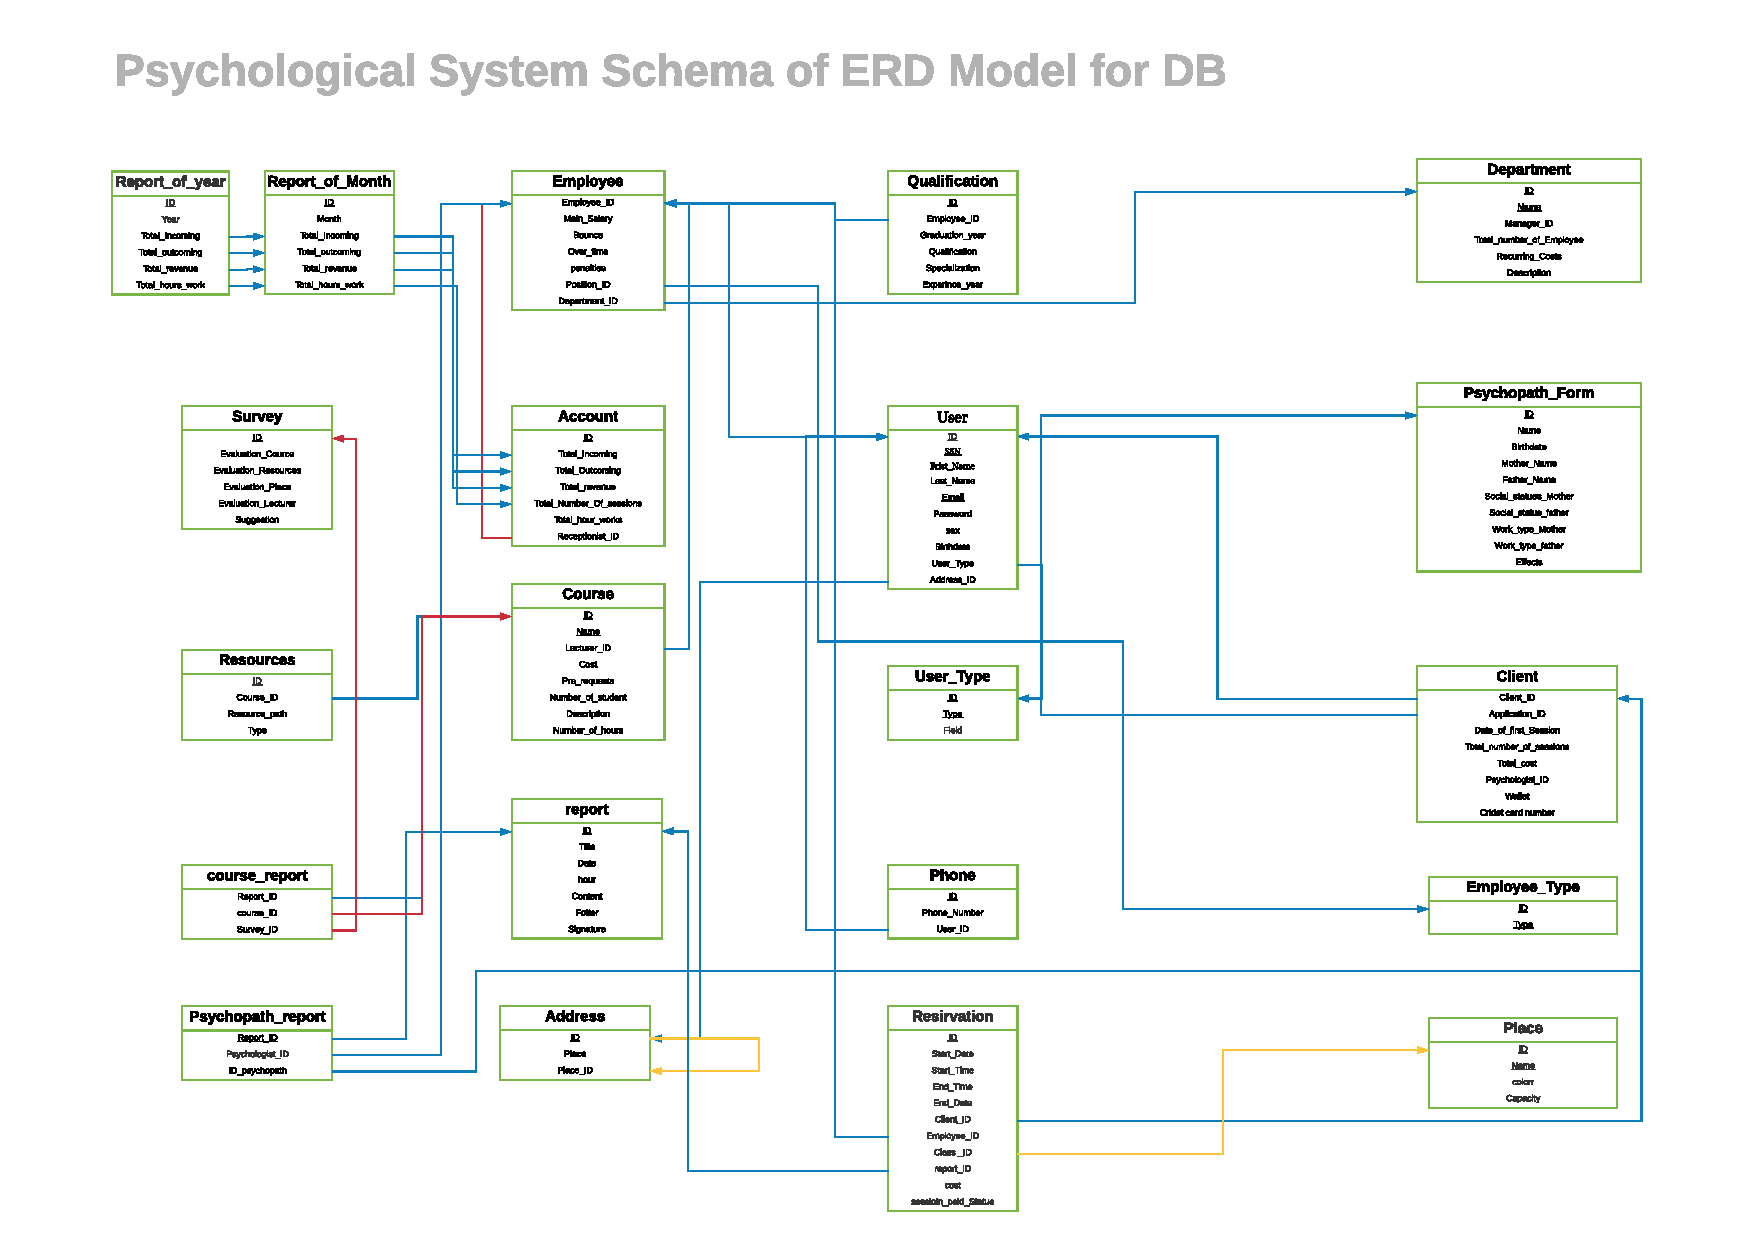
\includegraphics[width=\textwidth ,height=0.9\textheight ,scale=4]{Diagrams/Psychological_schema.pdf}
					\label{FIG:2.01}
				
								
				
			\subsection{Data flow diagram}
				\subsubsection{Context diagram}
					
						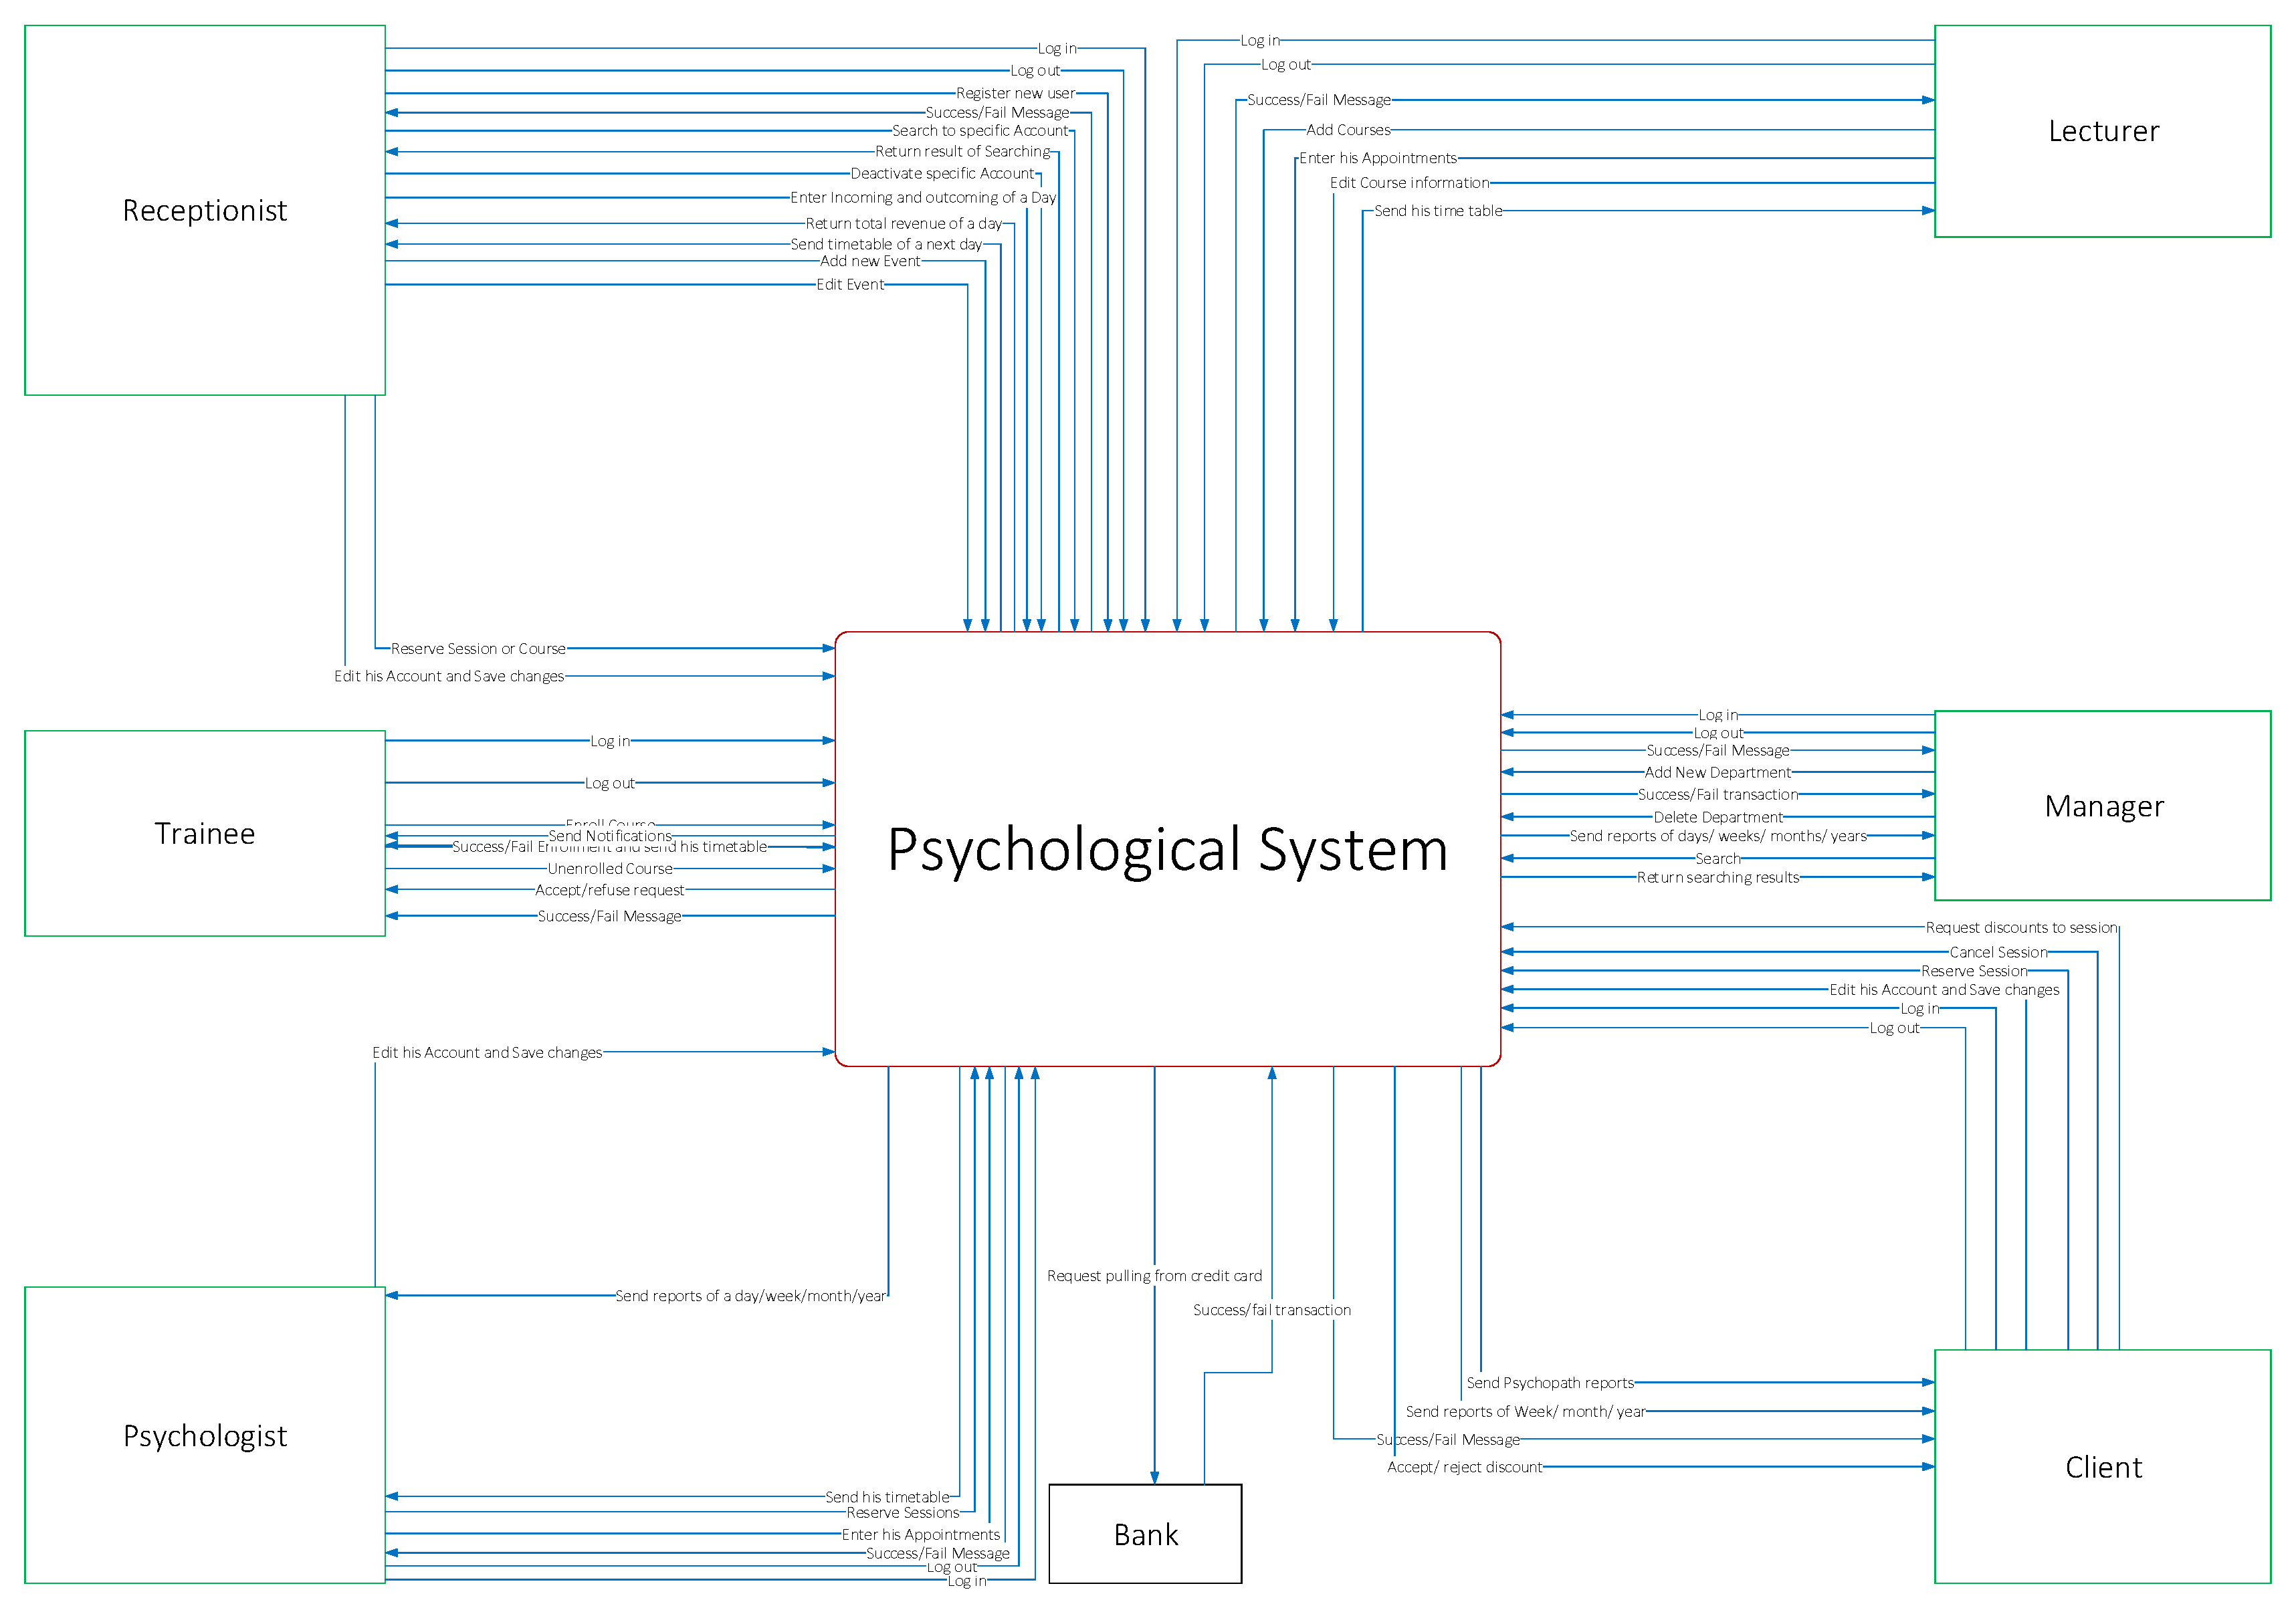
\includegraphics[width=\textwidth ,height=0.9\textheight ,scale=4]{Diagrams/Data-Flow_Context.pdf}
						\label{FIG:2.02}
					
					
				\subsubsection{level one}
					
						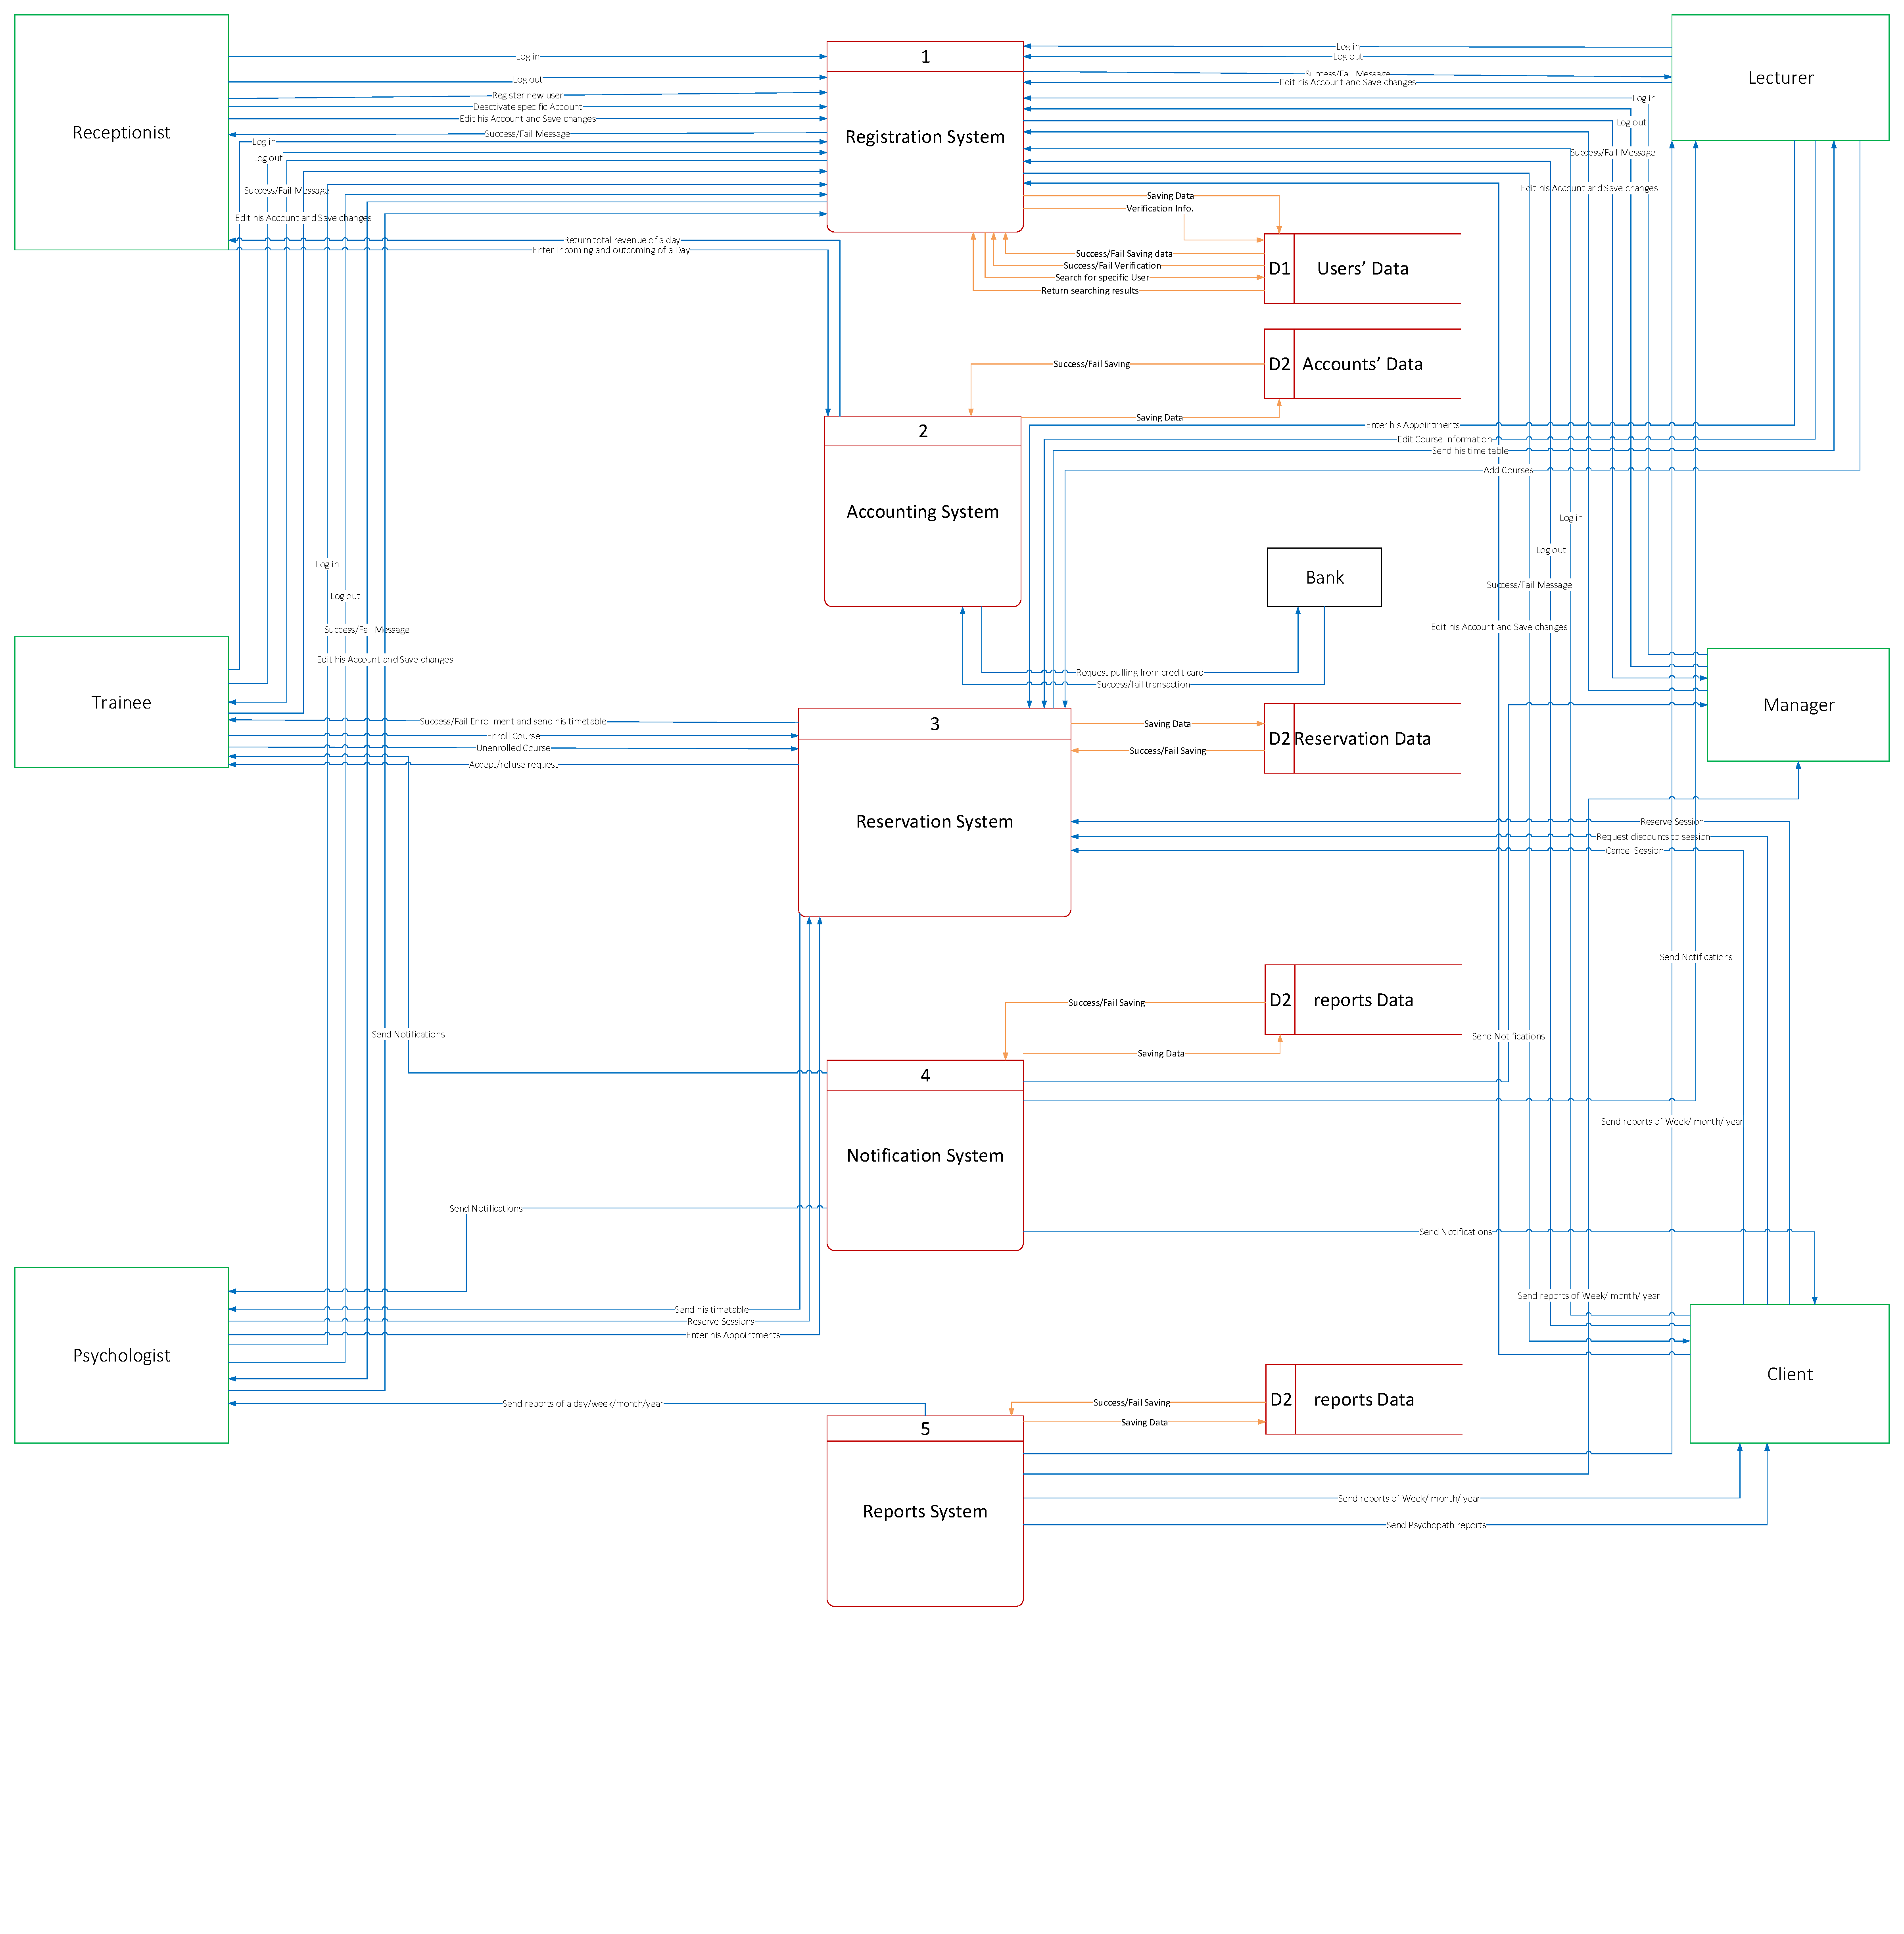
\includegraphics[width=\textwidth ,height=0.9\textheight ,scale=4]{Diagrams/Data-Flow_level0.pdf}
						\label{FIG:2.03}
					
					

				\subsection{Use case diagram}
				
					
						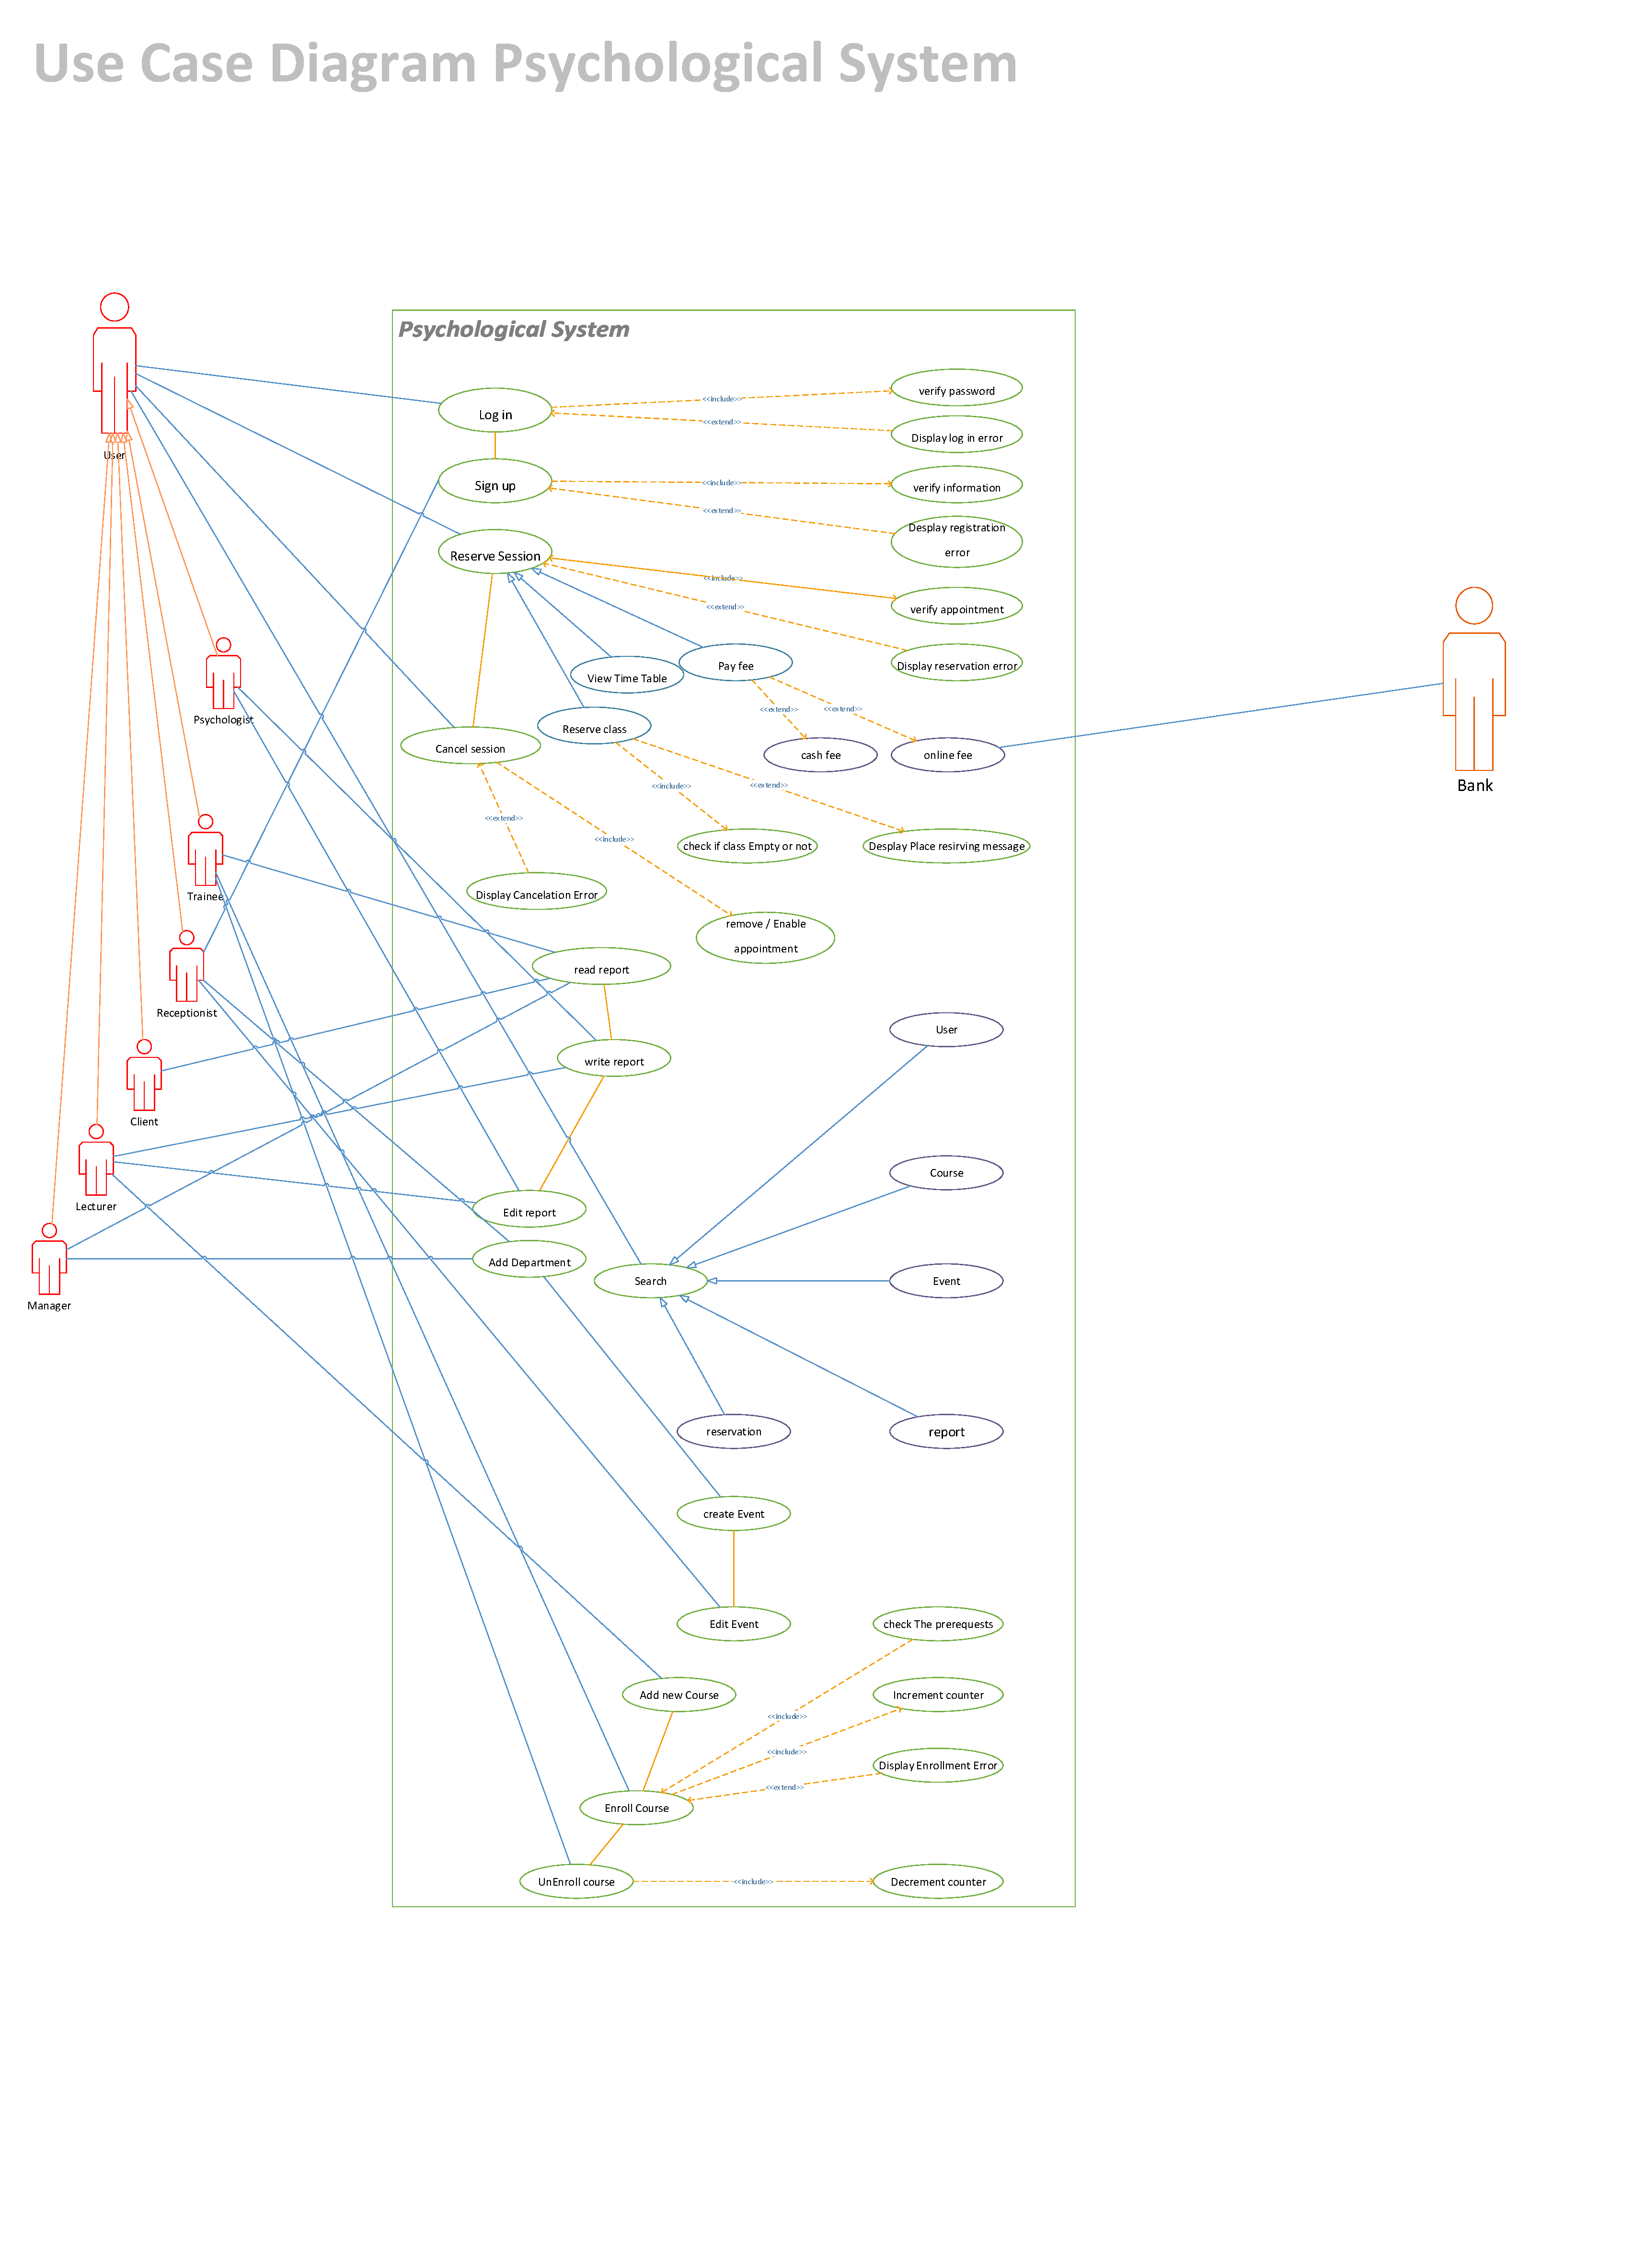
\includegraphics[width=\textwidth ,height=0.9\textheight ,scale=4]{Diagrams/use_case_psychological_system.pdf}
						\label{FIG:2.04}
					
						\subsubsection{Dictionary}
							\paragraph{The dictionary of use case created to describe use cases diagram we will see description to Registration use case \ref{table:Registration}, Log in use case \ref{table:LOG_IN}, Log out \ref{table:LOG_OUT},edit profile use case \ref{table:EDIT-PROFILE}, Forget Password \ref{table:FORGET-PASSWORD}, reserve event \ref{table:RESERVE-SESSION}, Cancel reservation \ref{table:CANCEL-RESERVATION}, read report use case \ref{table:READ-REPORT}, Write report use case \ref{table:WRITE-REPORT}, Edit report use case \ref{table:EDIT-REPORT}, Create new course use case \ref{table:CREATE-COURSE}}
%%%%%%%%%%%%%%%%%%%%%%%%%%%%%%%%%%%%%%%%%%%%%%%%%%%%%%%%%%%%%%%%%%%%%%%%%%%%%%%%%%%%%%%%%%%%%%%%%%%%%%%%%%%%%%%%%%%%%%%%%%%%%%%
%%%%%%%%%%%%%%%%%%%%%%%%%%%%%%%%%%%%%%%%%Registration%%%%%%%%%%%%%%%%%%%%%%%%%%%%%%%%%%%%%%%%%%%%%%%%%%%%%%%%%%%%%%%%%%%%%%%%%%
%%%%%%%%%%%%%%%%%%%%%%%%%%%%%%%%%%%%%%%%%%%%%%%%%%%%%%%%%%%%%%%%%%%%%%%%%%%%%%%%%%%%%%%%%%%%%%%%%%%%%%%%%%%%%%%%%%%%%%%%%%%%%%%

	\begin{center}
		\begin{table}[h!]
			\begin{tabular}{ | m{4cm} | m{10cm}| } 
				\hline
			 	\textbf{\large Name}& Sign Up\\
			 	
				\hline
			  	\textbf{\large Actors}& user(Receptionist, Manager)\\ 
								
				\hline
			  	\textbf{\large Description}& the user enters the website and then fills the required information from him and then an account is created for him on the site.\\
			  	 
				\hline
				\textbf{\large Data}&SSN, First Name, Last Name, Email, Password, Birth-date, User type, Address, phone Numbers \\ 
				
				\hline
				 \textbf{\large Pr-Condition}&user entering information into form \\
				
				\hline
				\textbf{\large Basic Flow}&\begin{enumerate}
				\item
					Open Home Page 
				\item
					User fills all basic information about him (first name ,Last name ,Job Title, Department, Picture)
				\item
					Click on create profile Button \end{enumerate}				 \\
				
				\hline
				\textbf{\large Alternative Flow}& If employee missed any information ,prompt him.\\ 
								
				\hline
				\textbf{\large Post Condition}& If The case completed Successfully, user has an account.\\ 
								
				\hline
				\textbf{\large Comments}& user must have  an email and code.\\ 
				\hline
			\end{tabular}
			\caption{Registration}
			\label{table:Registration}
		\end{table}
	\end{center}
%%%%%%%%%%%%%%%%%%%%%%%%%%%%%%%%%%%%%%%%%%%%%%%%%%%%%%%%%%%%%%%%%%%%%%%%%%%%%%%%%%%%%%%%%%%%%%%%%%%%%%%%%%%%%%%%%%%%%%%%%%%%%%%
%%%%%%%%%%%%%%%%%%%%%%%%%%%%%%%%%%%%%%%%%Log In%%%%%%%%%%%%%%%%%%%%%%%%%%%%%%%%%%%%%%%%%%%%%%%%%%%%%%%%%%%%%%%%%%%%%%%%%%%%%%%%
%%%%%%%%%%%%%%%%%%%%%%%%%%%%%%%%%%%%%%%%%%%%%%%%%%%%%%%%%%%%%%%%%%%%%%%%%%%%%%%%%%%%%%%%%%%%%%%%%%%%%%%%%%%%%%%%%%%%%%%%%%%%%%%
	\begin{center}
		\begin{table}[h!]
			\begin{tabular}{ | m{4cm} | m{10cm}| } 
				\hline
			 	\textbf{\large Name}& Log In\\ 
				\hline
			  	\textbf{\large Actors}& user(Receptionist, Lecturer, Client, Trainee, Psychologist, Manager)\\ 
				\hline
			  	\textbf{\large Description}& user enters the needed information to enter his account on site.\\ 
				\hline
				\textbf{\large Data}& user-name Or Email , password\\ 
				\hline
				\textbf{\large Pr-Condition}&user entering information into form \\
				\hline
				\textbf{\large Basic Flow}&\begin{enumerate}
				\item
					Open Home Page 
				\item
					Enter Email as User-name and Biometric Iris as Password
				\item
					Click on Log-in Button \end{enumerate}				 \\
				\hline
				\textbf{\large Alternative Flow}& If The User-name or Password is incorrect The User is prompted to re-enter Information again.\\ 
				\hline
				\textbf{\large Post Condition}& If The case completed Successfully, user can access.\\ 
				\hline
				\textbf{\large Comments}& user must have an account on site.\\ 
				\hline
			\end{tabular}
			\caption{Log-In}
			\label{table:LOG_IN}
		\end{table}
	\end{center}
%%%%%%%%%%%%%%%%%%%%%%%%%%%%%%%%%%%%%%%%%%%%%%%%%%%%%%%%%%%%%%%%%%%%%%%%%%%%%%%%%%%%%%%%%%%%%%%%%%%%%%%%%%%%%%%%%%%%%%%%%%%%%%%
%%%%%%%%%%%%%%%%%%%%%%%%%%%%%%%%%%%%%%%%%Log Out%%%%%%%%%%%%%%%%%%%%%%%%%%%%%%%%%%%%%%%%%%%%%%%%%%%%%%%%%%%%%%%%%%%%%%%%%%%%%%%
%%%%%%%%%%%%%%%%%%%%%%%%%%%%%%%%%%%%%%%%%%%%%%%%%%%%%%%%%%%%%%%%%%%%%%%%%%%%%%%%%%%%%%%%%%%%%%%%%%%%%%%%%%%%%%%%%%%%%%%%%%%%%%%
	\begin{center}
		\begin{table}[h!]
			\begin{tabular}{ | m{4cm} | m{10cm}| } 
				\hline
			 	\textbf{\large Name}& Log Out\\ 
				\hline
			  	\textbf{\large Actors}& user(Receptionist, Lecturer, Client, Trainee, Psychologist, Manager)\\ 
				\hline
			  	\textbf{\large Description}& user press log-out button to leave account.\\ 
				\hline
				\textbf{\large Data}& None.\\ 
				\hline
				 \textbf{\large Pr-Condition}& user press log-out button. \\ 
				\hline
				\textbf{\large Basic Flow}&\begin{enumerate}
				\item
					Press Setting button 
				\item
					press Log out button \end{enumerate}\\
					\hline
				\textbf{\large Alternative Flow}& If connection errors\\ 
				\hline
				\textbf{\large Post Condition}& user leaves his account must re-log-in.\\ 
				\hline
				\textbf{\large Comments}& user must be logged in to account on site.\\ 
				\hline
			\end{tabular}
			\caption{Log-Out}
			\label{table:LOG_OUT}
		\end{table}
	\end{center}
	
%%%%%%%%%%%%%%%%%%%%%%%%%%%%%%%%%%%%%%%%%%%%%%%%%%%%%%%%%%%%%%%%%%%%%%%%%%%%%%%%%%%%%%%%%%%%%%%%%%%%%%%%%%%%%%%%%%%%%%%%%%%%%%%
%%%%%%%%%%%%%%%%%%%%%%%%%%%%%%%%%%%%%%%%%Edit profile%%%%%%%%%%%%%%%%%%%%%%%%%%%%%%%%%%%%%%%%%%%%%%%%%%%%%%%%%%%%%%%%%%%%%%%%%%
%%%%%%%%%%%%%%%%%%%%%%%%%%%%%%%%%%%%%%%%%%%%%%%%%%%%%%%%%%%%%%%%%%%%%%%%%%%%%%%%%%%%%%%%%%%%%%%%%%%%%%%%%%%%%%%%%%%%%%%%%%%%%%%

	\begin{center}
		\begin{table}[h!]
			\begin{tabular}{ | m{4cm} | m{10cm}| } 
				\hline
			 	\textbf{\large Name}& Edit Profile\\
			 	
				\hline
			  	\textbf{\large Actors}& user(Receptionist, Lecturer, Client, Trainee, Psychologist, Manager)\\ 
								
				\hline
			  	\textbf{\large Description}& the user wants to edit some information like change password or email address...etc.\\
			  	 
				\hline
				\textbf{\large Data}&SSN, First Name, Last Name, Email, Password, Birth-date, User type, Address, phone Numbers \\ 
				
				\hline
				 \textbf{\large Pr-Condition}& Must have an account in the web \\
				
				\hline
				\textbf{\large Basic Flow}&\begin{enumerate}
				\item
					Open profile
				\item
					choose setting list then press on Edit my profile
				\item
					after Editing press on save changes \end{enumerate}				 \\
				
				\hline
				\textbf{\large Alternative Flow}& If User did not press on save changes after Editing.\\ 
								
				\hline
				\textbf{\large Post Condition}& Editing profile.\\ 
								
				\hline
				\textbf{\large Comments}& user must have  an email and code.\\ 
				\hline
			\end{tabular}
			\caption{Edit Profile}
			\label{table:EDIT-PROFILE}
		\end{table}
	\end{center}
	
%%%%%%%%%%%%%%%%%%%%%%%%%%%%%%%%%%%%%%%%%%%%%%%%%%%%%%%%%%%%%%%%%%%%%%%%%%%%%%%%%%%%%%%%%%%%%%%%%%%%%%%%%%%%%%%%%%%%%%%%%%%%%%%
%%%%%%%%%%%%%%%%%%%%%%%%%%%%%%%%%%%%%%%%%Forget password%%%%%%%%%%%%%%%%%%%%%%%%%%%%%%%%%%%%%%%%%%%%%%%%%%%%%%%%%%%%%%%%%%%%%%%
%%%%%%%%%%%%%%%%%%%%%%%%%%%%%%%%%%%%%%%%%%%%%%%%%%%%%%%%%%%%%%%%%%%%%%%%%%%%%%%%%%%%%%%%%%%%%%%%%%%%%%%%%%%%%%%%%%%%%%%%%%%%%%%

	\begin{center}
		\begin{table}[h!]
			\begin{tabular}{ | m{4cm} | m{10cm}| } 
				\hline
			 	\textbf{\large Name}& Forget Password\\
			 	
				\hline
			  	\textbf{\large Actors}& user(Receptionist, Lecturer, Client, Trainee, Psychologist, Manager)\\ 
								
				\hline
			  	\textbf{\large Description}& the user wants to recovering his account and he forget his password.\\
			  	 
				\hline
				\textbf{\large Data}&Email address, phone number, and last password he know\\ 
				
				\hline
				 \textbf{\large Pr-Condition}& Must have an account in the web \\
				
				\hline
				\textbf{\large Basic Flow}&\begin{enumerate}
				\item
					Open home page
				\item
					choose log in the forget password
				\item
					Enter activation key
				\item
					Enter new password  \end{enumerate}				 \\
				
				\hline
				\textbf{\large Alternative Flow}& If User forget most information about his account.\\ 
								
				\hline
				\textbf{\large Post Condition}& recovering account.\\ 
								
				\hline
				\textbf{\large Comments}& user must have an account on site.\\ 
				\hline
			\end{tabular}
			\caption{Forget Password}
			\label{table:FORGET-PASSWORD}
		\end{table}
	\end{center}
%%%%%%%%%%%%%%%%%%%%%%%%%%%%%%%%%%%%%%%%%Reserve Event%%%%%%%%%%%%%%%%%%%%%%%%%%%%%%%%%%%%%%%%%%%%%%%%%%%%%%%%%%%%%%%%%%%%%%%
%%%%%%%%%%%%%%%%%%%%%%%%%%%%%%%%%%%%%%%%%%%%%%%%%%%%%%%%%%%%%%%%%%%%%%%%%%%%%%%%%%%%%%%%%%%%%%%%%%%%%%%%%%%%%%%%%%%%%%%%%%%%%%%
	\begin{center}
		\begin{table}[h!]
			\begin{tabular}{ | m{4cm} | m{10cm}| } 
				\hline
			 	\textbf{\large Name}& Reserve Session\\ 
				\hline
			  	\textbf{\large Actors}& user(Receptionist, Lecturer, Trainee ,Client, Psychologist)\\ 
				\hline
			  	\textbf{\large Description}& user enters the needed information to reserve Session.\\ 
				\hline
				\textbf{\large Data}& Start Date, End Date, Start hour, End hour, Psychologist, Cost, Paid way.\\ 
				\hline
				 \textbf{\large Pr-Condition}& User press to reserve Session button and enter the information needed then press submit to save the reservation. \\ 
				\hline
				\textbf{\large Basic Flow}&\begin{enumerate}
				\item
					Press reservation button 
				\item
					Enter required Data
				\item 
					press submit \end{enumerate}\\
					\hline
				\textbf{\large Alternative Flow}& If user Enter invalid data or did not press submit button\\ 
				\hline
				\textbf{\large Post Condition}& Create Appointment to him with the Specific Psychologist.\\ 
				\hline
				\textbf{\large Comments}& user must have an account on site.\\ 
				\hline
			\end{tabular}
			\caption{Reserve Session}
			\label{table:RESERVE-SESSION}
		\end{table}
	\end{center}
%%%%%%%%%%%%%%%%%%%%%%%%%%%%%%%%%%%%%%%%%Cancel resrvation%%%%%%%%%%%%%%%%%%%%%%%%%%%%%%%%%%%%%%%%%%%%%%%%%%%%%%%%%%%%%%%%%%%%%
%%%%%%%%%%%%%%%%%%%%%%%%%%%%%%%%%%%%%%%%%%%%%%%%%%%%%%%%%%%%%%%%%%%%%%%%%%%%%%%%%%%%%%%%%%%%%%%%%%%%%%%%%%%%%%%%%%%%%%%%%%%%%%%
	\begin{center}
		\begin{table}[h!]
			\begin{tabular}{ | m{4cm} | m{10cm}| } 
				\hline
			 	\textbf{\large Name}& Cancel reservation\\ 
				\hline
			  	\textbf{\large Actors}& user(Receptionist, Lecturer, Trainee ,Client, Psychologist)\\ 
				\hline
			  	\textbf{\large Description}& user wants to cancel session or course.\\ 
				\hline
				\textbf{\large Data}& None.\\ 
				\hline
				 \textbf{\large Pr-Condition}& User reserve session or course. \\ 
				\hline
				\textbf{\large Basic Flow}&\begin{enumerate}
				\item
					Press List of reservation
				\item
					choose an event that will cancel
				\item 
					press cancel button \end{enumerate}\\
					\hline
				\textbf{\large Alternative Flow}& If user wants to cancel after 24 hours to session, or if he cancel after preparing the tools of courses.\\ 
				\hline
				\textbf{\large Post Condition}& Cancel reservation of course or session.\\ 
				\hline
				\textbf{\large Comments}& user must have an account on site.\\ 
				\hline
			\end{tabular}
			\caption{Cancel reservation}
			\label{table:CANCEL-RESERVATION}
		\end{table}
	\end{center}
	
%%%%%%%%%%%%%%%%%%%%%%%%%%%%%%%%%%%%%%%%%read report%%%%%%%%%%%%%%%%%%%%%%%%%%%%%%%%%%%%%%%%%%%%%%%%%%%%%%%%%%%%%%%%%%%%%%%%%%%
%%%%%%%%%%%%%%%%%%%%%%%%%%%%%%%%%%%%%%%%%%%%%%%%%%%%%%%%%%%%%%%%%%%%%%%%%%%%%%%%%%%%%%%%%%%%%%%%%%%%%%%%%%%%%%%%%%%%%%%%%%%%%%%
	\begin{center}
		\begin{table}[h!]
			\begin{tabular}{ | m{4cm} | m{10cm}| } 
				\hline
			 	\textbf{\large Name}& Read report\\ 
				\hline
			  	\textbf{\large Actors}& user(Manager, Receptionist, Lecturer, Trainee ,Client, Psychologist)\\ 
				\hline
			  	\textbf{\large Description}& all users read them reports in the system.\\ 
				\hline
				\textbf{\large Data}& ID, Title, Date, Time, body, footer, signature.\\ 
				\hline
				 \textbf{\large Pr-Condition}& found Writing reports. \\ 
				\hline
				\textbf{\large Basic Flow}&\begin{enumerate}
				\item
					Press on List of reports
				\item
					choose a report that will read it
				\item 
					press on it \end{enumerate}\\
					\hline
				\textbf{\large Alternative Flow}& If report had damaged, or not permission for you.\\ 
				\hline
				\textbf{\large Post Condition}& opening report as read only.\\ 
				\hline
				\textbf{\large Comments}& user must have an account on site, and have some activities on site.\\ 
				\hline
			\end{tabular}
			\caption{read report}
			\label{table:READ-REPORT}
		\end{table}
	\end{center}
	
%%%%%%%%%%%%%%%%%%%%%%%%%%%%%%%%%%%%%%%%%Write report%%%%%%%%%%%%%%%%%%%%%%%%%%%%%%%%%%%%%%%%%%%%%%%%%%%%%%%%%%%%%%%%%%%%%%%%%%
%%%%%%%%%%%%%%%%%%%%%%%%%%%%%%%%%%%%%%%%%%%%%%%%%%%%%%%%%%%%%%%%%%%%%%%%%%%%%%%%%%%%%%%%%%%%%%%%%%%%%%%%%%%%%%%%%%%%%%%%%%%%%%%
	\begin{center}
		\begin{table}[h!]
			\begin{tabular}{ | m{4cm} | m{10cm}| } 
				\hline
			 	\textbf{\large Name}& Write report\\ 
				\hline
			  	\textbf{\large Actors}& user(Lecturer, Psychologist)\\ 
				\hline
			  	\textbf{\large Description}& lecturer and Psychologist Write reports of courses or sessions, or the system generate some reports.\\ 
				\hline
				\textbf{\large Data}& ID, Title, Date, Time, body, footer, signature.\\ 
				\hline
				 \textbf{\large Pr-Condition}& Psychologist or lecturer has session or course. \\ 
				\hline
				\textbf{\large Basic Flow}&\begin{enumerate}
				\item
					Press on List of reports
				\item
					press on crate button
				\item 
					press on save report button \end{enumerate}\\
					\hline
				\textbf{\large Alternative Flow}& If Psychologist or lecturer did not press on save report button, or Enter invalid data.\\ 
				\hline
				\textbf{\large Post Condition}& Creating report.\\ 
				\hline
				\textbf{\large Comments}& user must have an account on site, and have some activities on site.\\ 
				\hline
			\end{tabular}
			\caption{Write report}
			\label{table:WRITE-REPORT}
		\end{table}
	\end{center}
	
%%%%%%%%%%%%%%%%%%%%%%%%%%%%%%%%%%%%%%%%%Edit report%%%%%%%%%%%%%%%%%%%%%%%%%%%%%%%%%%%%%%%%%%%%%%%%%%%%%%%%%%%%%%%%%%%%%%%%%%%
%%%%%%%%%%%%%%%%%%%%%%%%%%%%%%%%%%%%%%%%%%%%%%%%%%%%%%%%%%%%%%%%%%%%%%%%%%%%%%%%%%%%%%%%%%%%%%%%%%%%%%%%%%%%%%%%%%%%%%%%%%%%%%%
	\begin{center}
		\begin{table}[h!]
			\begin{tabular}{ | m{4cm} | m{10cm}| } 
				\hline
			 	\textbf{\large Name}& Edit report\\ 
				\hline
			  	\textbf{\large Actors}& user(Lecturer, Psychologist)\\ 
				\hline
			  	\textbf{\large Description}& lecturer and Psychologist wants edit reports of courses or sessions for his reasons.\\ 
				\hline
				\textbf{\large Data}& ID, Title, Date, Time, body, footer, signature.\\ 
				\hline
				 \textbf{\large Pr-Condition}& Psychologist or lecturer create report previously. \\ 
				\hline
				\textbf{\large Basic Flow}&\begin{enumerate}
				\item
					Press on List of reports
				\item
					choose report that will Edit it
				\item 
					press on it
				\item
					then press on save report \end{enumerate}\\
					\hline
				\textbf{\large Alternative Flow}& If Psychologist or lecturer did not press on save report button, or Enter invalid data.\\ 
				\hline
				\textbf{\large Post Condition}& editing report.\\ 
				\hline
				\textbf{\large Comments}& user must have an account on site, and have some activities on site.\\ 
				\hline
			\end{tabular}
			\caption{Edit report}
			\label{table:EDIT-REPORT}
		\end{table}
	\end{center}
%%%%%%%%%%%%%%%%%%%%%%%%%%%%%%%%%%%%%%%%%Create New Course%%%%%%%%%%%%%%%%%%%%%%%%%%%%%%%%%%%%%%%%%%%%%%%%%%%%%%%%%%%%%%%%%%%%%
%%%%%%%%%%%%%%%%%%%%%%%%%%%%%%%%%%%%%%%%%%%%%%%%%%%%%%%%%%%%%%%%%%%%%%%%%%%%%%%%%%%%%%%%%%%%%%%%%%%%%%%%%%%%%%%%%%%%%%%%%%%%%%%
	\begin{center}
		\begin{table}[h!]
			\begin{tabular}{ | m{4cm} | m{10cm}| } 
				\hline
			 	\textbf{\large Name}& Create new course\\ 
				\hline
			  	\textbf{\large Actors}& user(Lecturer)\\ 
				\hline
			  	\textbf{\large Description}& lecturer  wants to create Course on the site.\\ 
				\hline
				\textbf{\large Data}& ID, Name, Cost, prerequisites, Description, hours.\\ 
				\hline
				 \textbf{\large Pr-Condition}& lecturer's account activated. \\ 
				\hline
				\textbf{\large Basic Flow}&\begin{enumerate}
				\item
					Press on create Course
				\item
					enter required data
				\item
					press on submit button \end{enumerate}\\
					\hline
				\textbf{\large Alternative Flow}& If lecturer did not press on submit button after creating course, or the course previously created on the system.\\ 
				\hline
				\textbf{\large Post Condition}& Added course.\\ 
				\hline
				\textbf{\large Comments}& user must have an account on site, and have some activities on site.\\ 
				\hline
			\end{tabular}
			\caption{Create New Course}
			\label{table:CREATE-COURSE}
		\end{table}
	\end{center}
	
	\clearpage
					\subsection{Class diagram}
						\subsubsection{Diagram}
						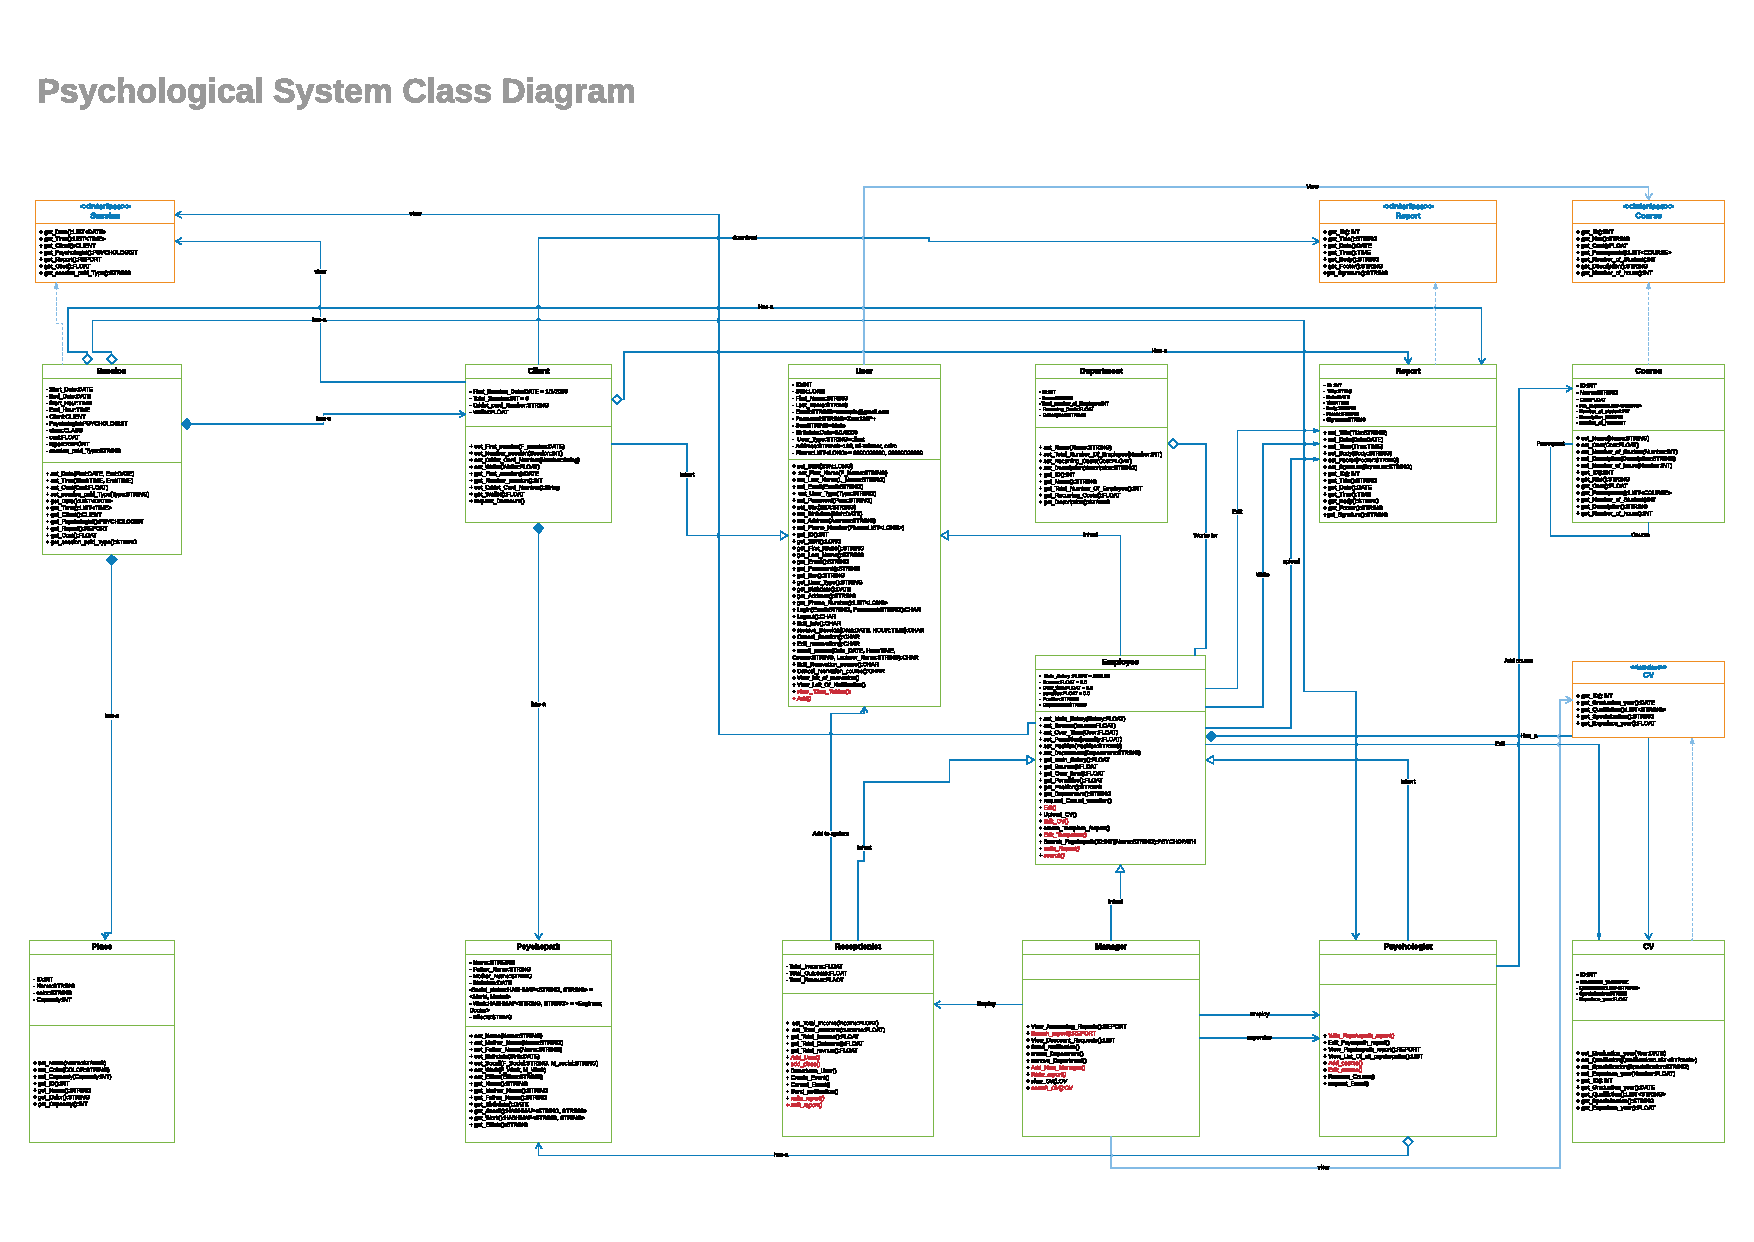
\includegraphics[width=\textwidth ,height=0.9\textheight ,scale=4]{Diagrams/Class_Diagram_for_Psychological_System.pdf}	
						\label{FIG:2.05}
						
					\subsection{Activity Diagram}
						
							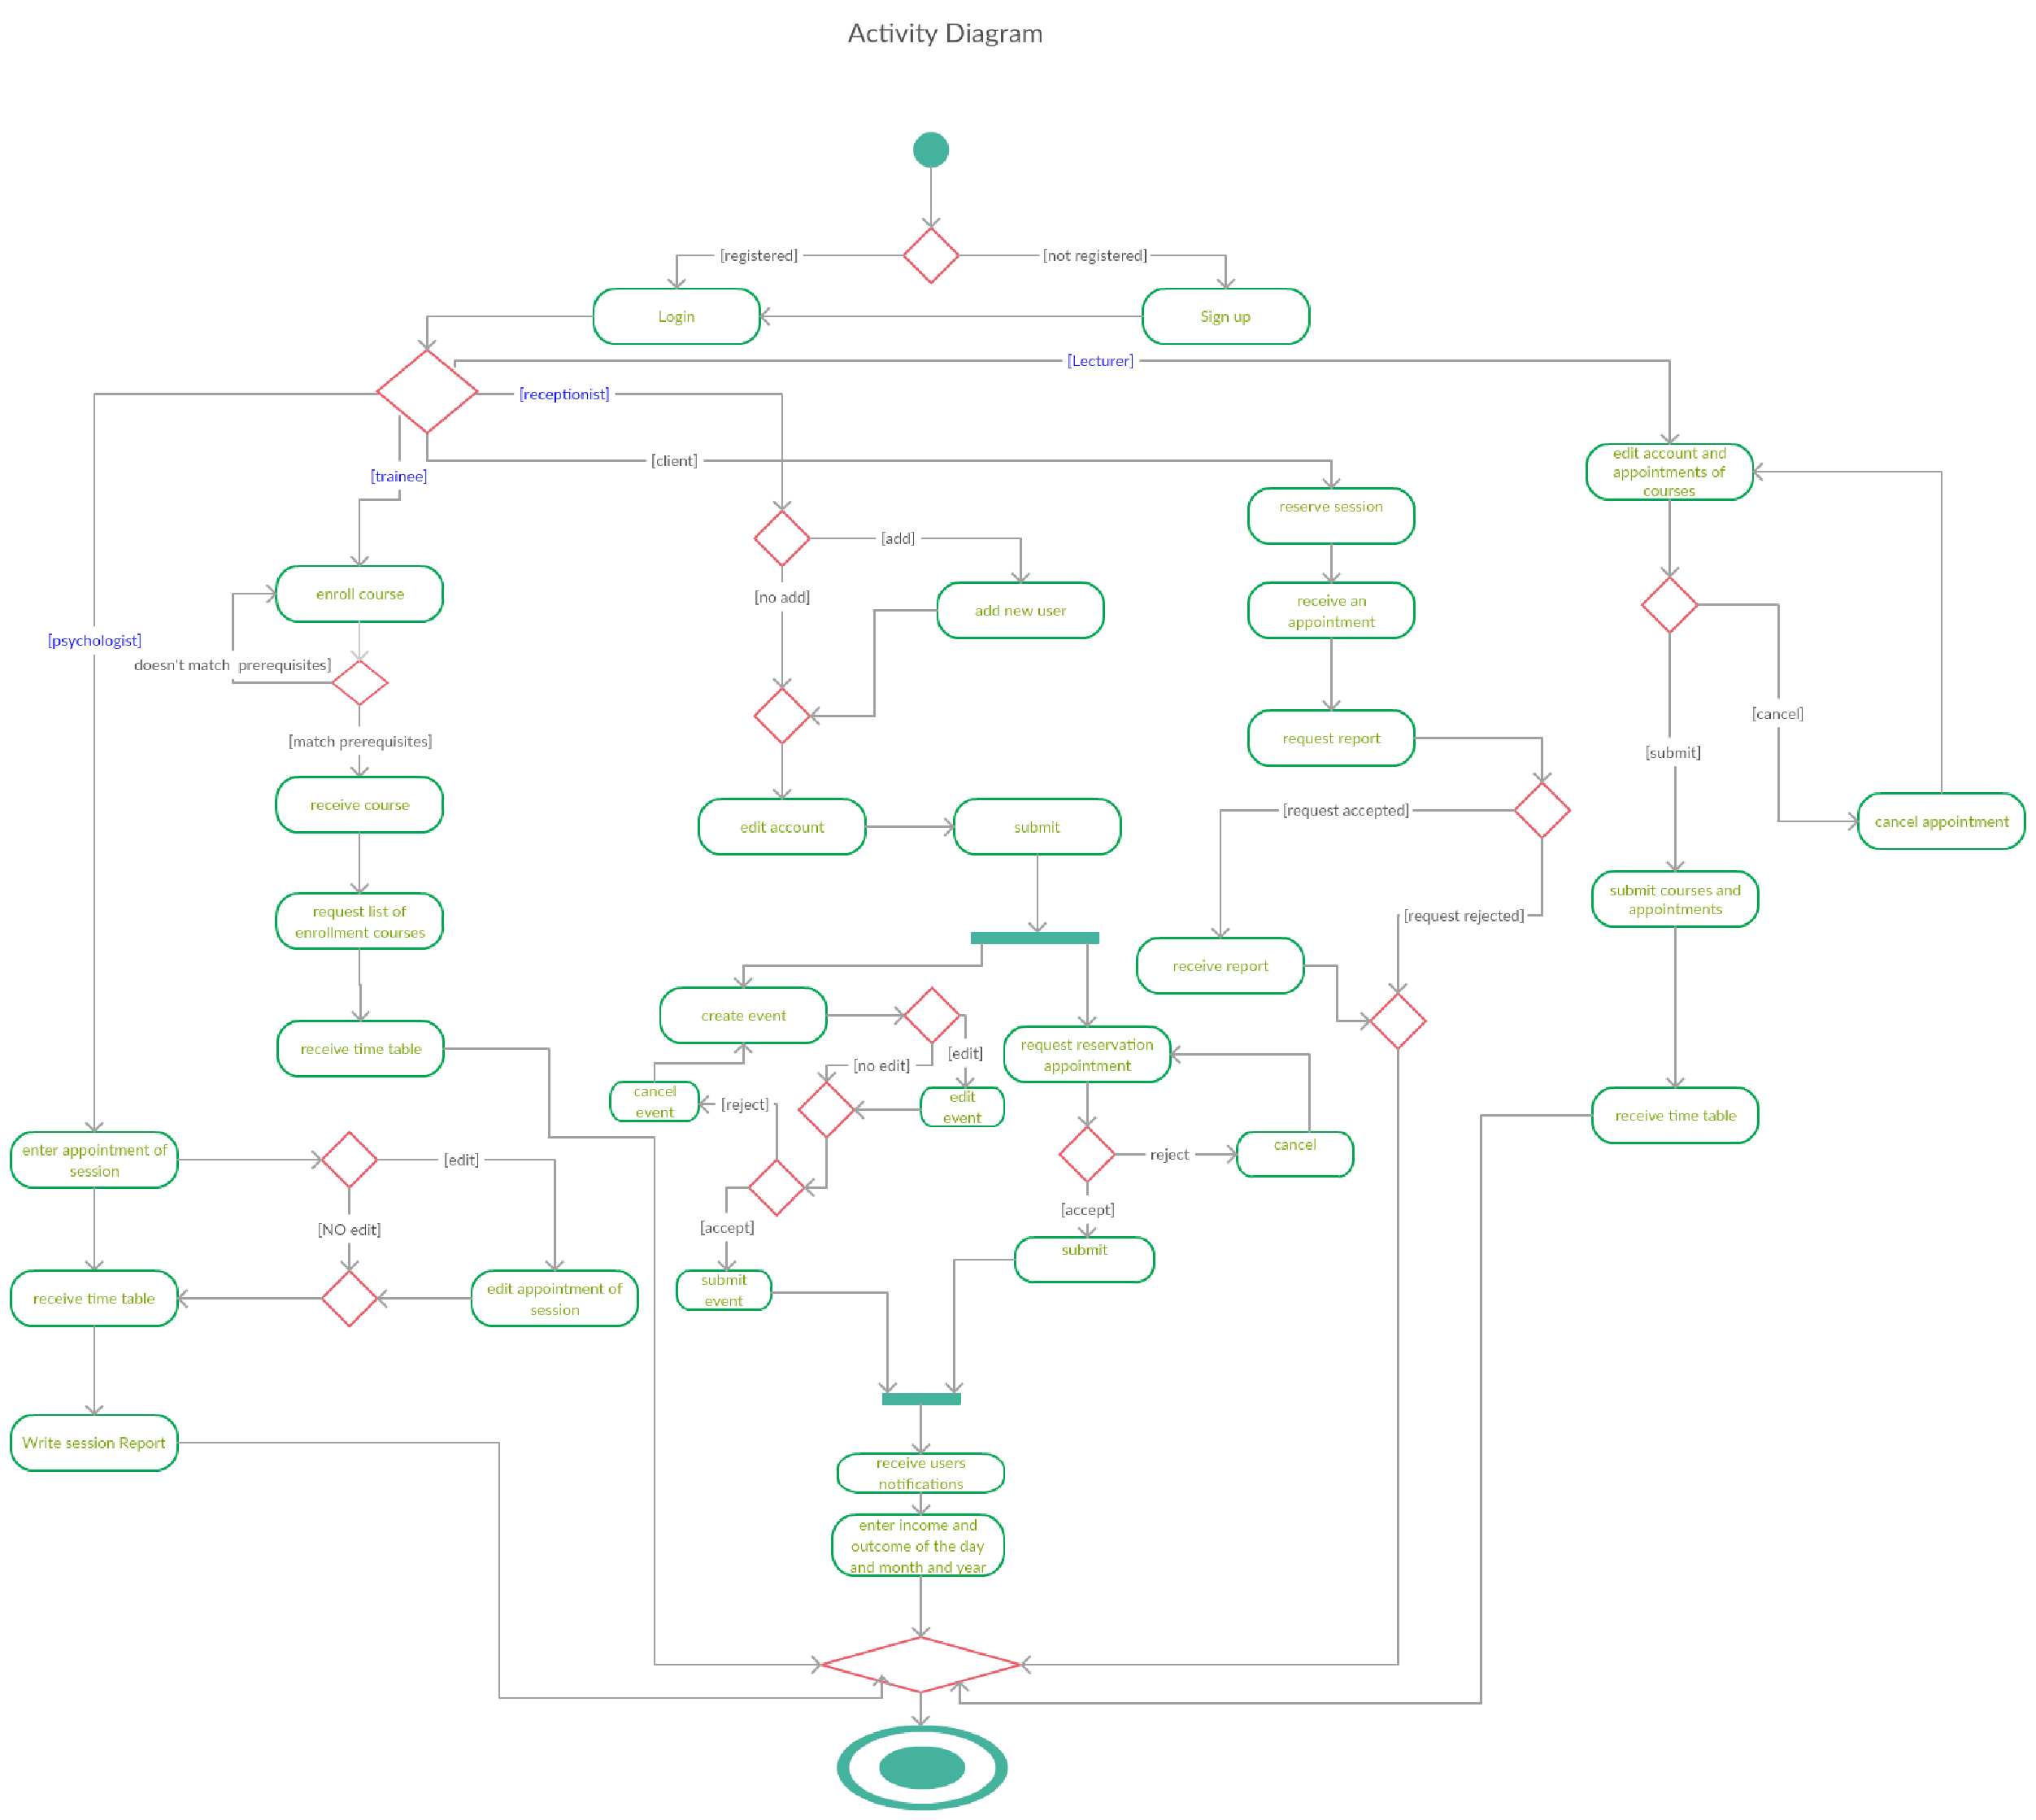
\includegraphics[width=\textwidth ,height=0.9\textheight ,scale=4]{Diagrams/Activity_Of_Psychological_System.pdf}
							\label{FIG:2.06}
						
					
					
						
					\subsection{Sequence Diagram}
						\subsubsection{Appointment reservation}
							
								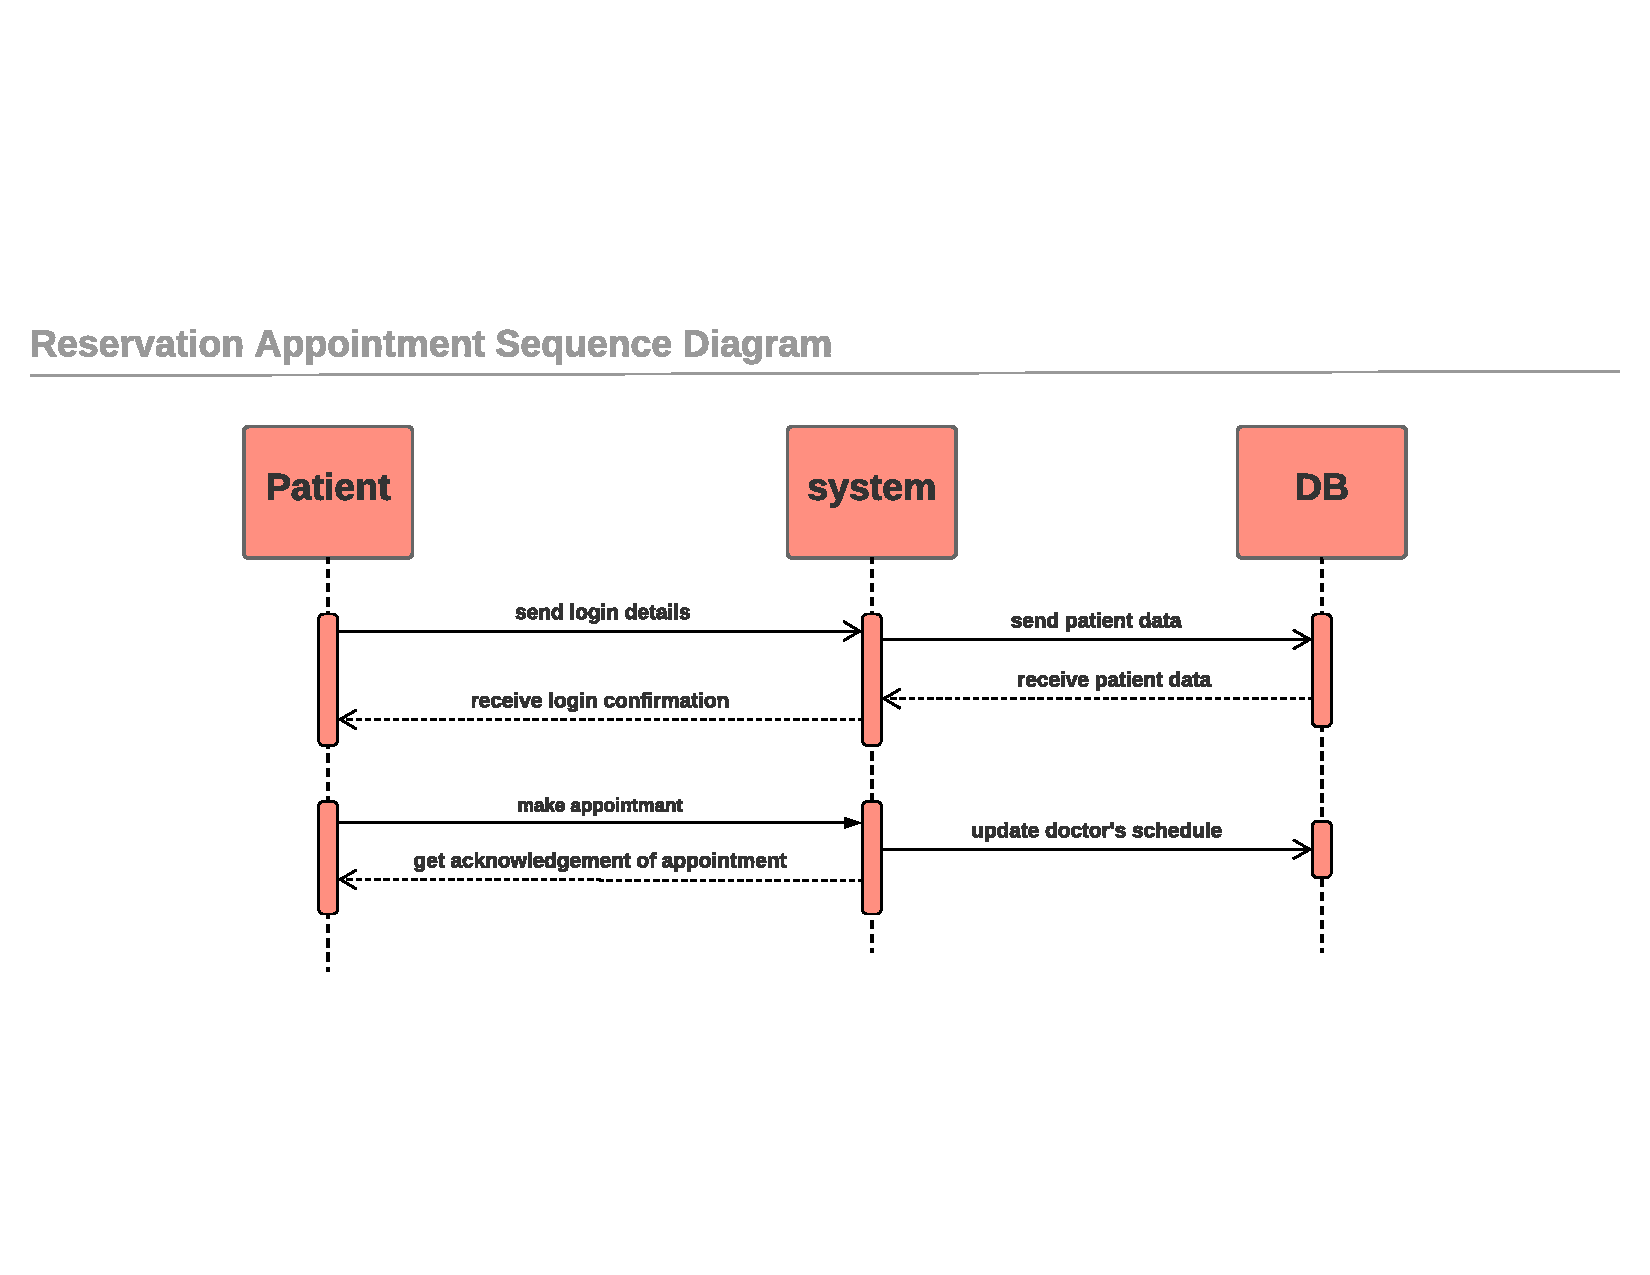
\includegraphics[width=\textwidth ,height=0.4\textheight ,scale=4]{Diagrams/sequence_diagram/appointment_reservation.pdf}
								\label{FIG:2.07}
							
							
						
						\subsubsection{Appointment cancellation}
							
								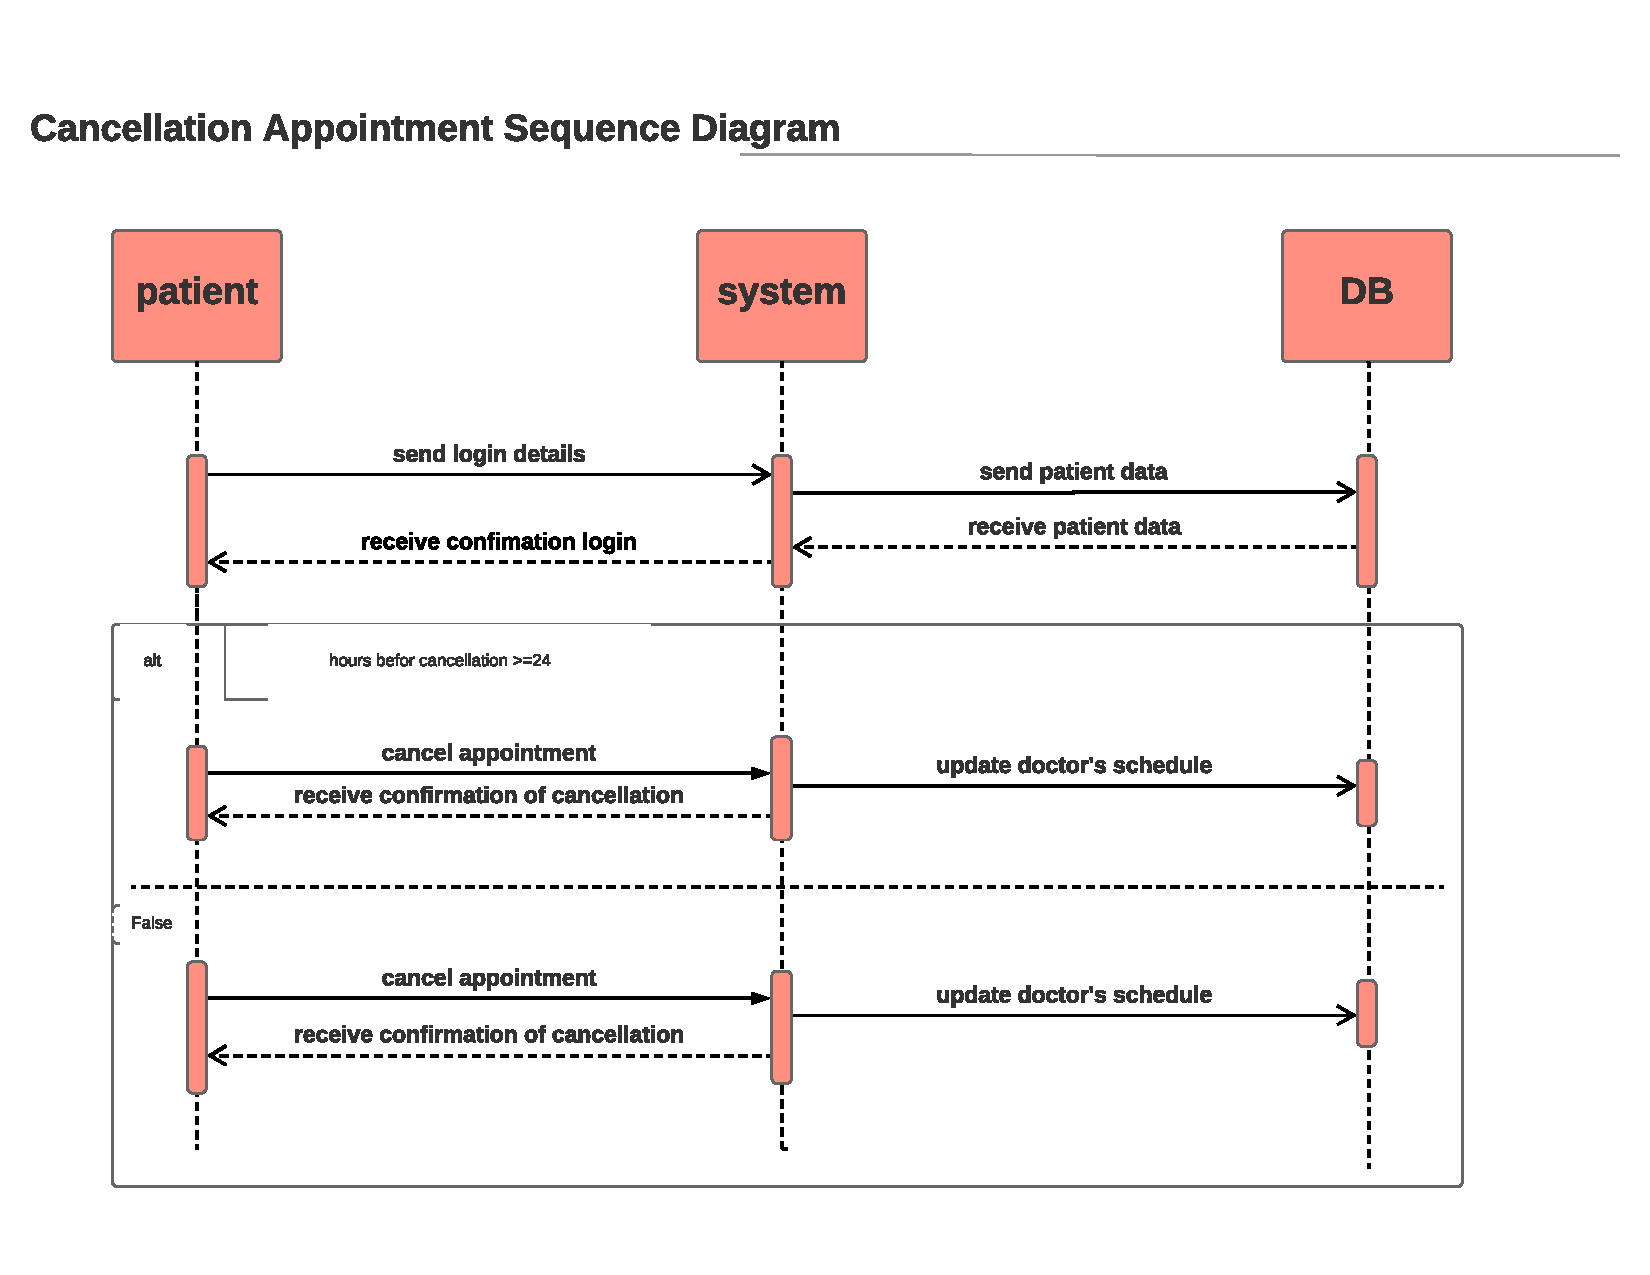
\includegraphics[width=\textwidth ,height=0.4\textheight ,scale=4]{Diagrams/sequence_diagram/appointment_cancellation.pdf}
								\label{FIG:2.08}
							
							
							
						\subsubsection{Psychologist}
							
								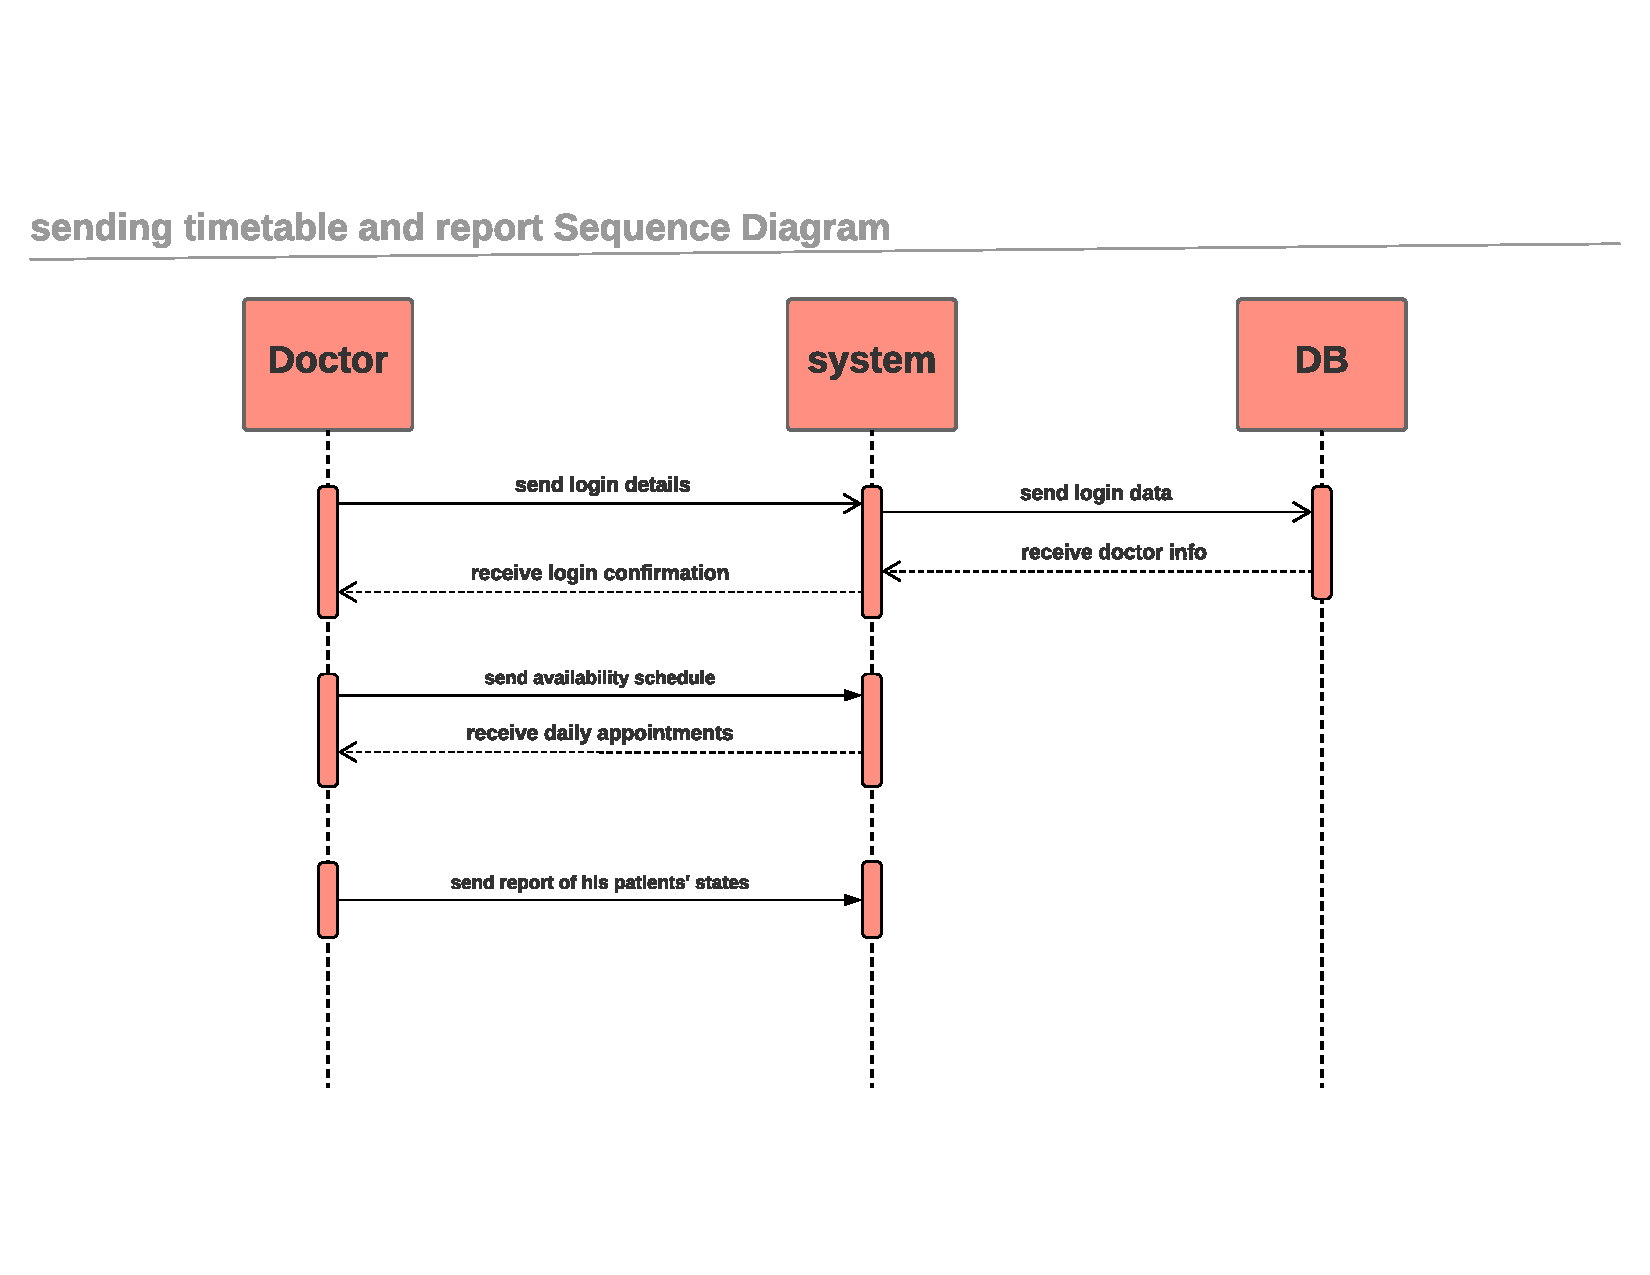
\includegraphics[width=\textwidth ,height=0.4\textheight ,scale=4]{Diagrams/sequence_diagram/doctor_sequence_diagram.pdf}
								\label{FIG:2.09}
							
							
							
						\subsubsection{Enroll Courses}
							
								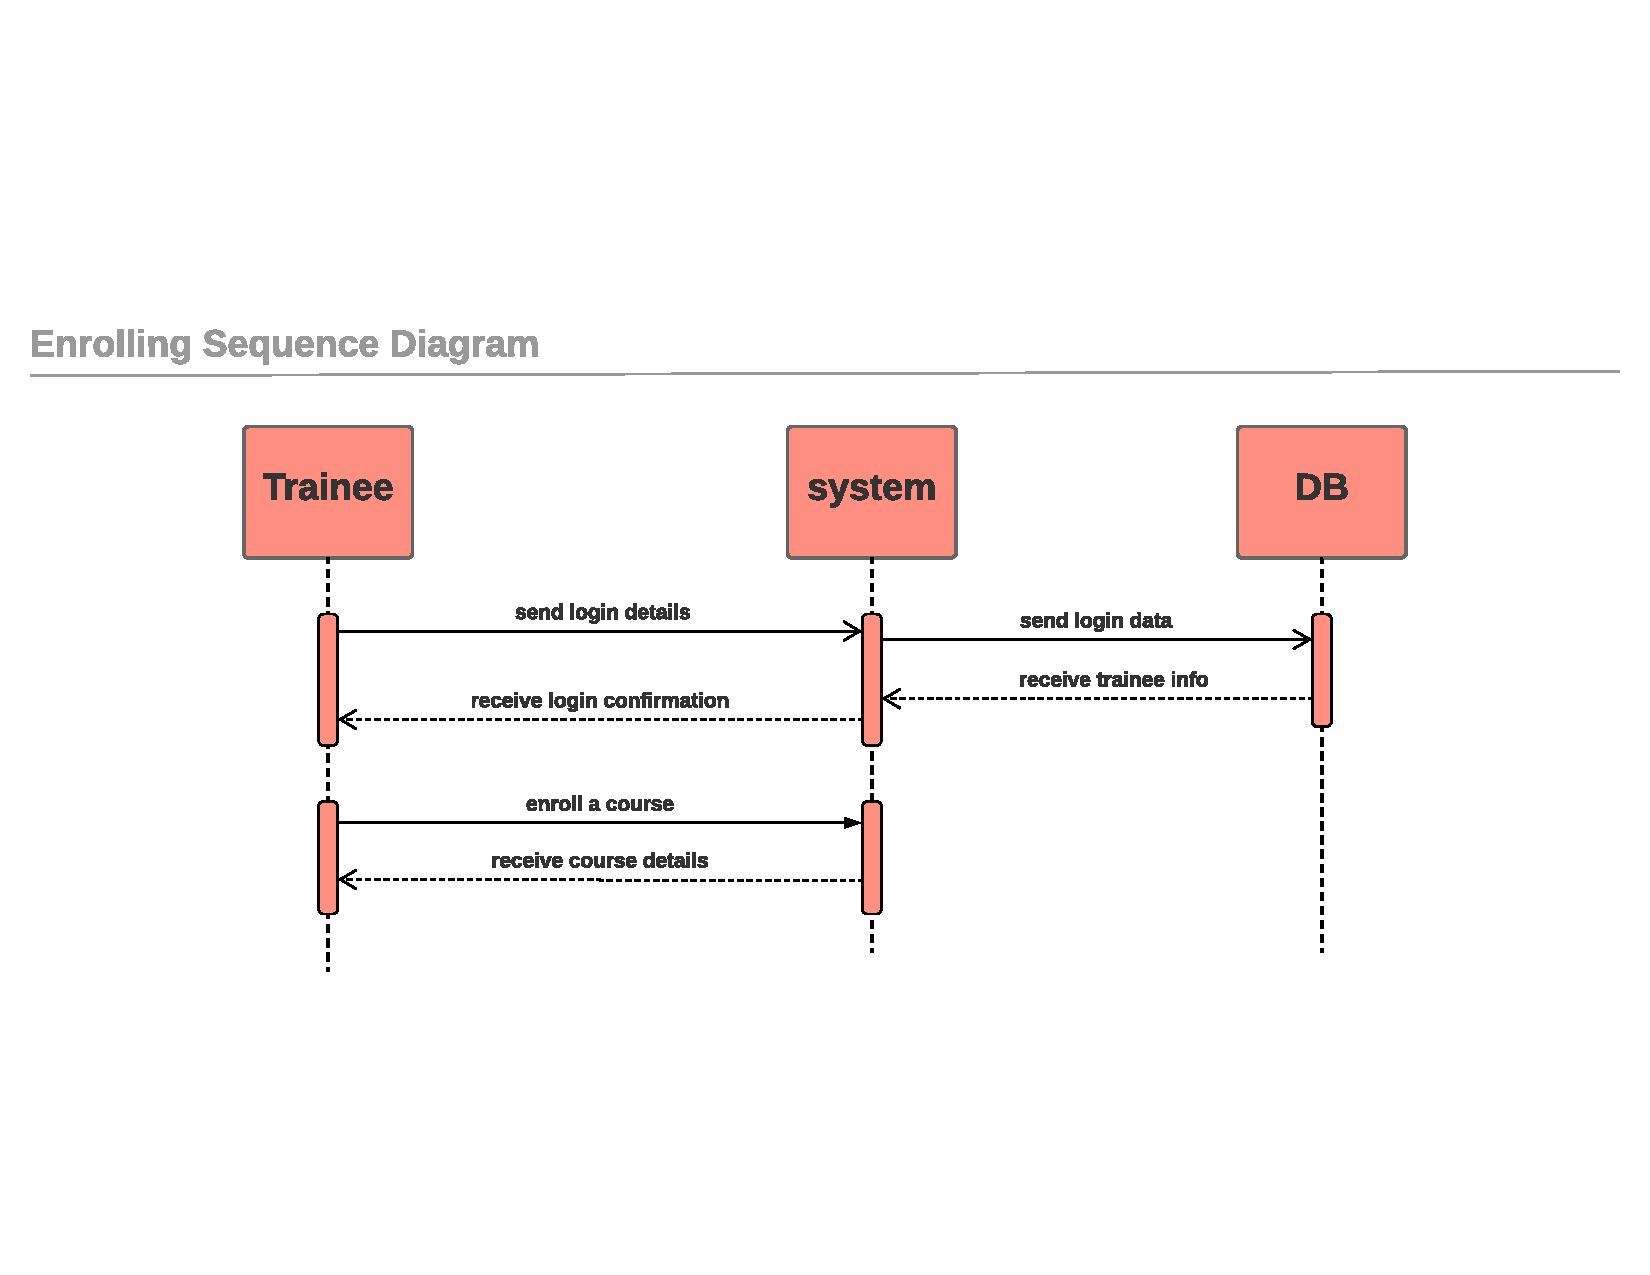
\includegraphics[width=\textwidth ,height=0.4\textheight ,scale=4]{Diagrams/sequence_diagram/enrolling.pdf}
								\label{FIG:2.10}
							
							
							
						\subsubsection{Add Courses}
							
								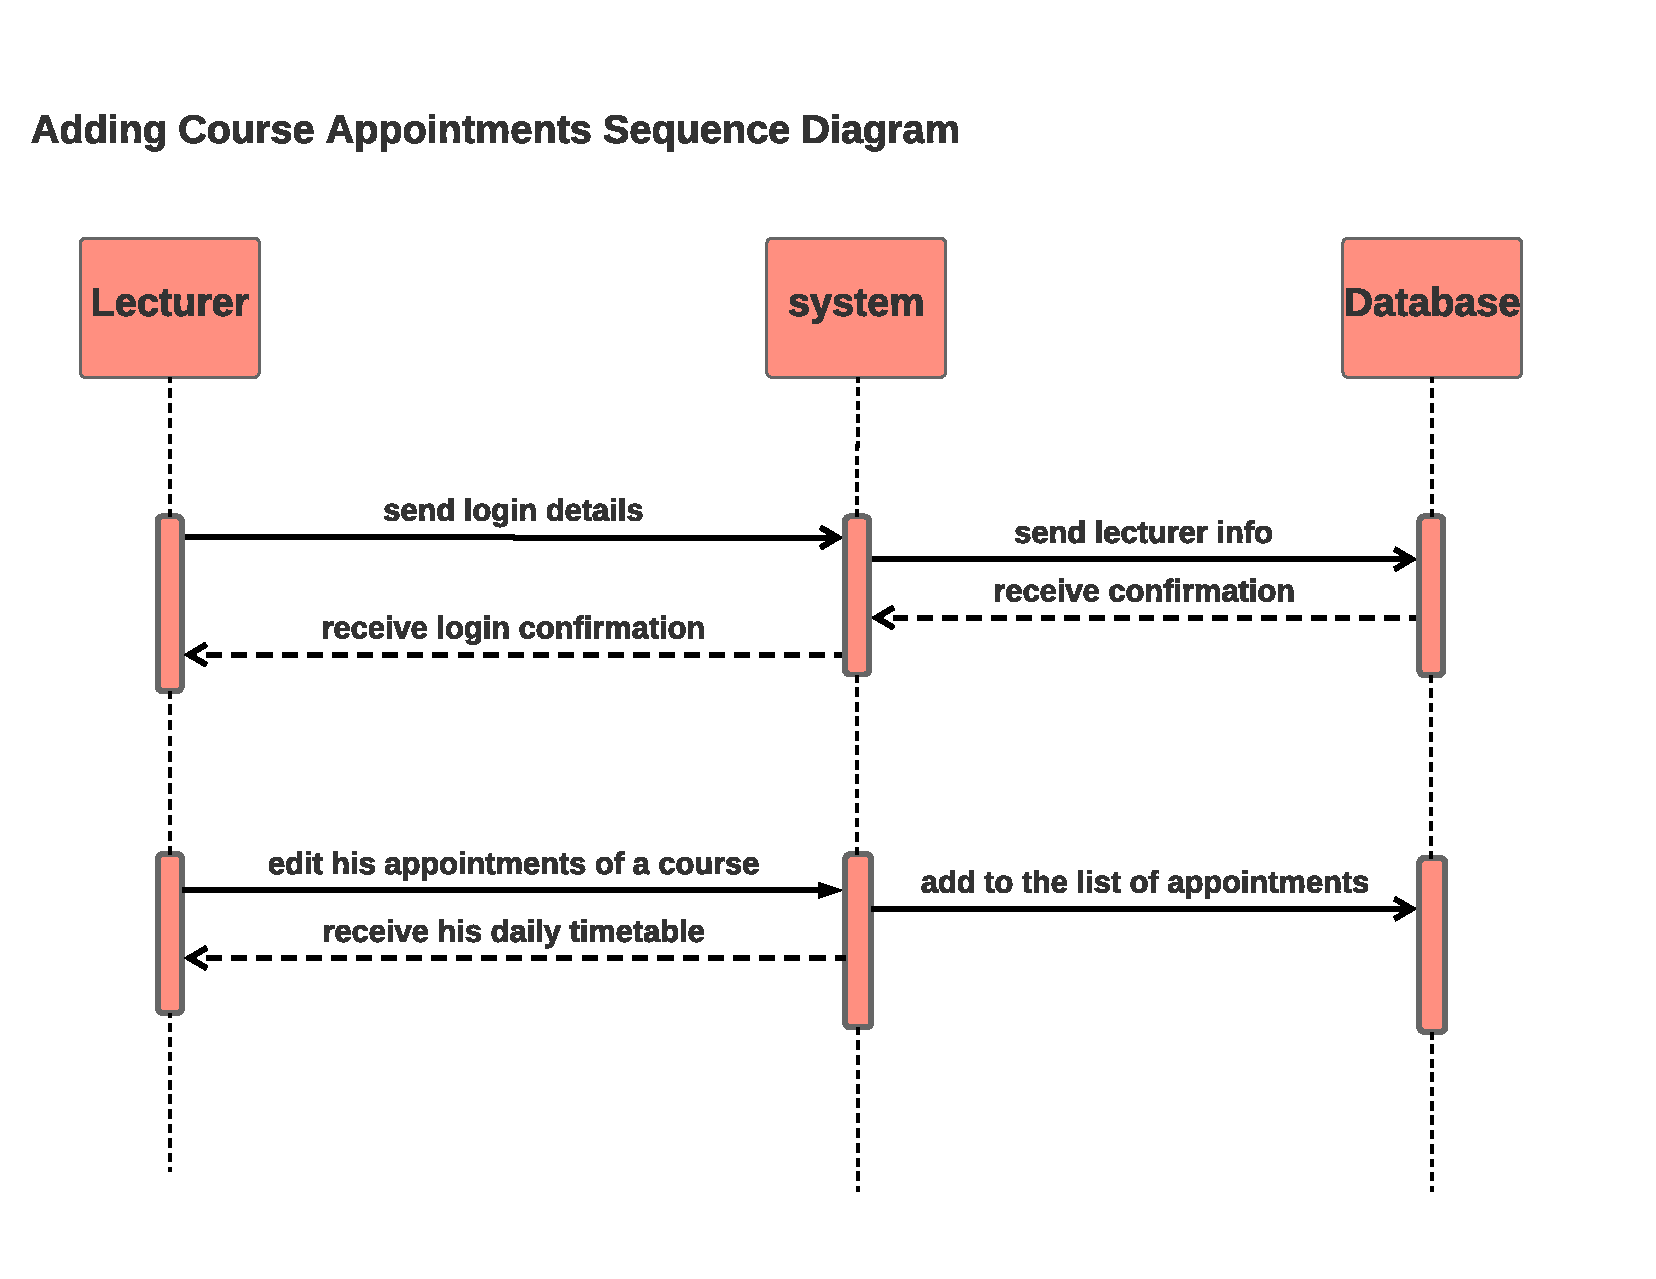
\includegraphics[width=\textwidth ,height=0.4\textheight ,scale=4]{Diagrams/sequence_diagram/Adding_course_lecturer.pdf}
								\label{FIG:2.11}
							
							
							
						\subsubsection{Unroll Courses}
							
								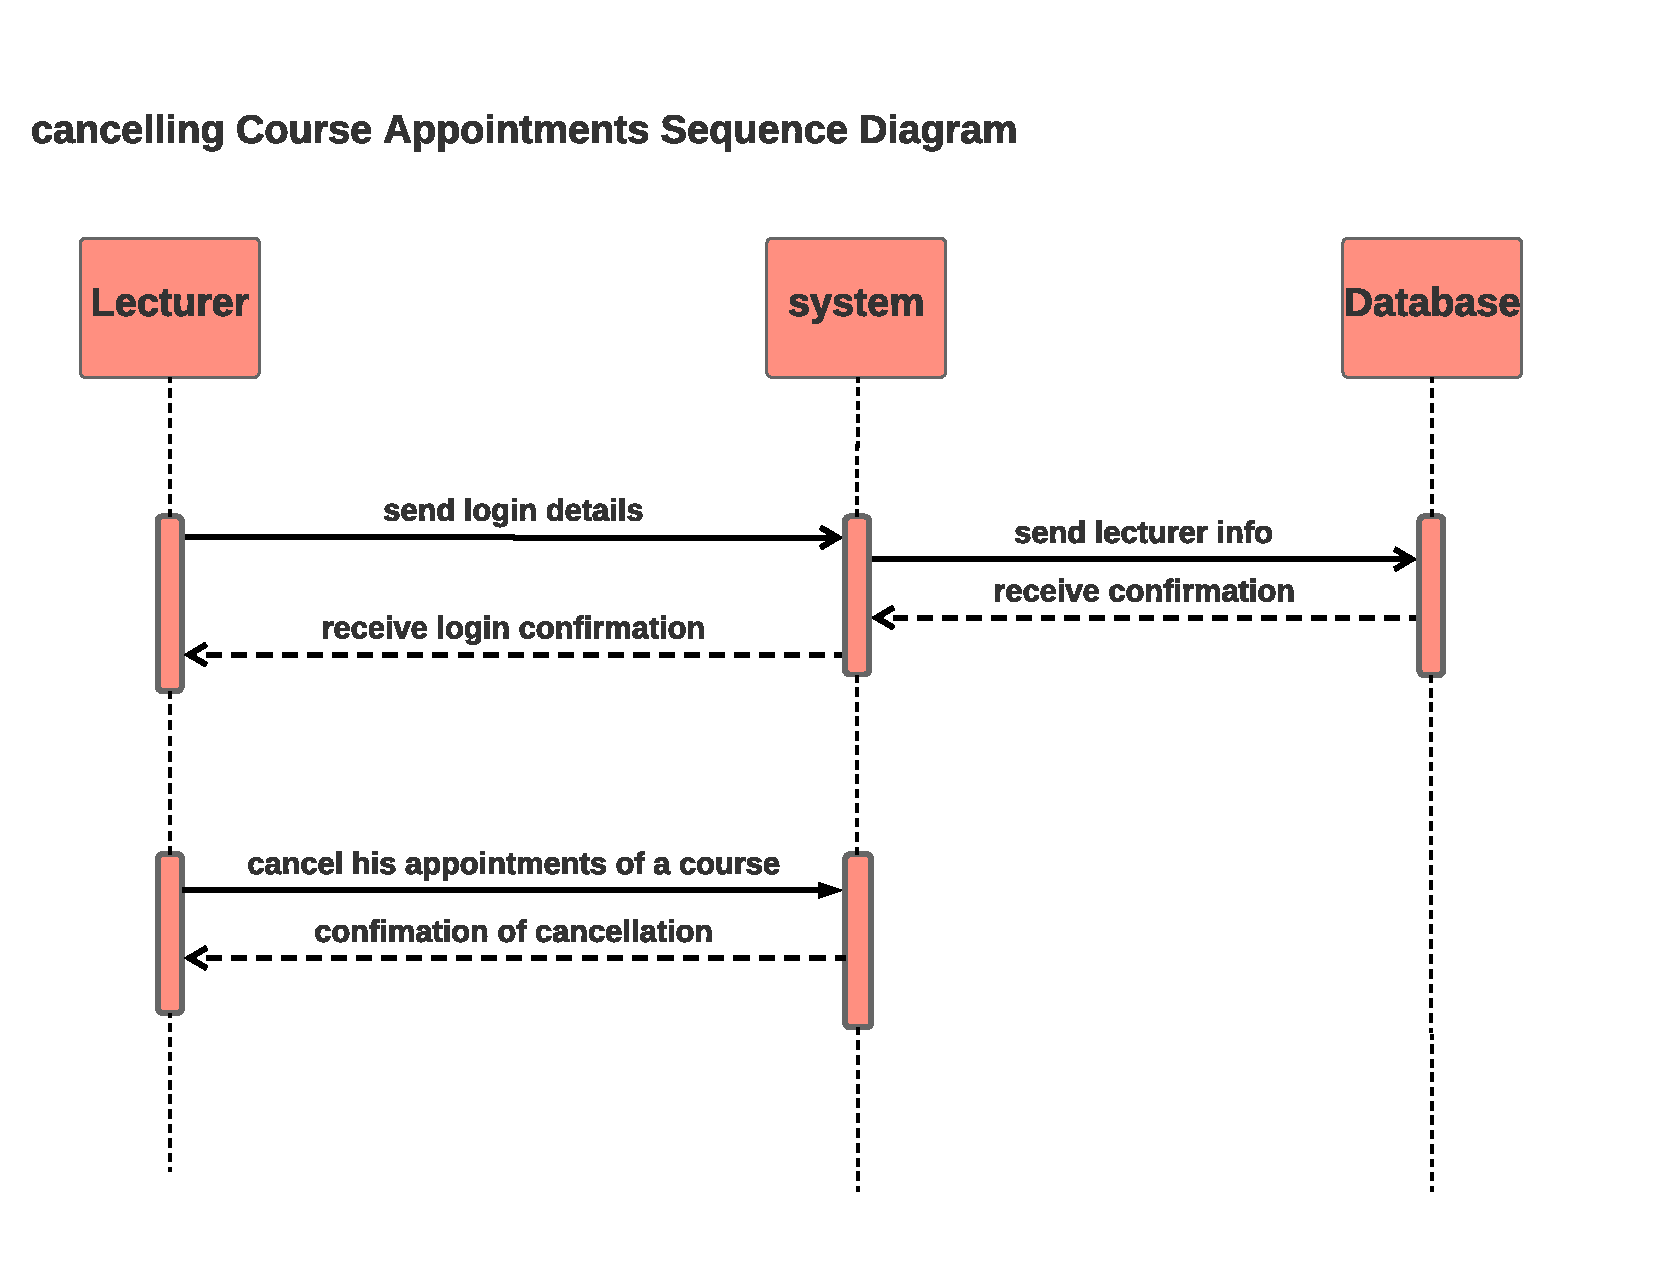
\includegraphics[width=\textwidth ,height=0.4\textheight ,scale=4]{Diagrams/sequence_diagram/cancel_course_lecturer.pdf}
								\label{FIG:2.12}
							
							
							
						\subsubsection{Manager request reports}
							
								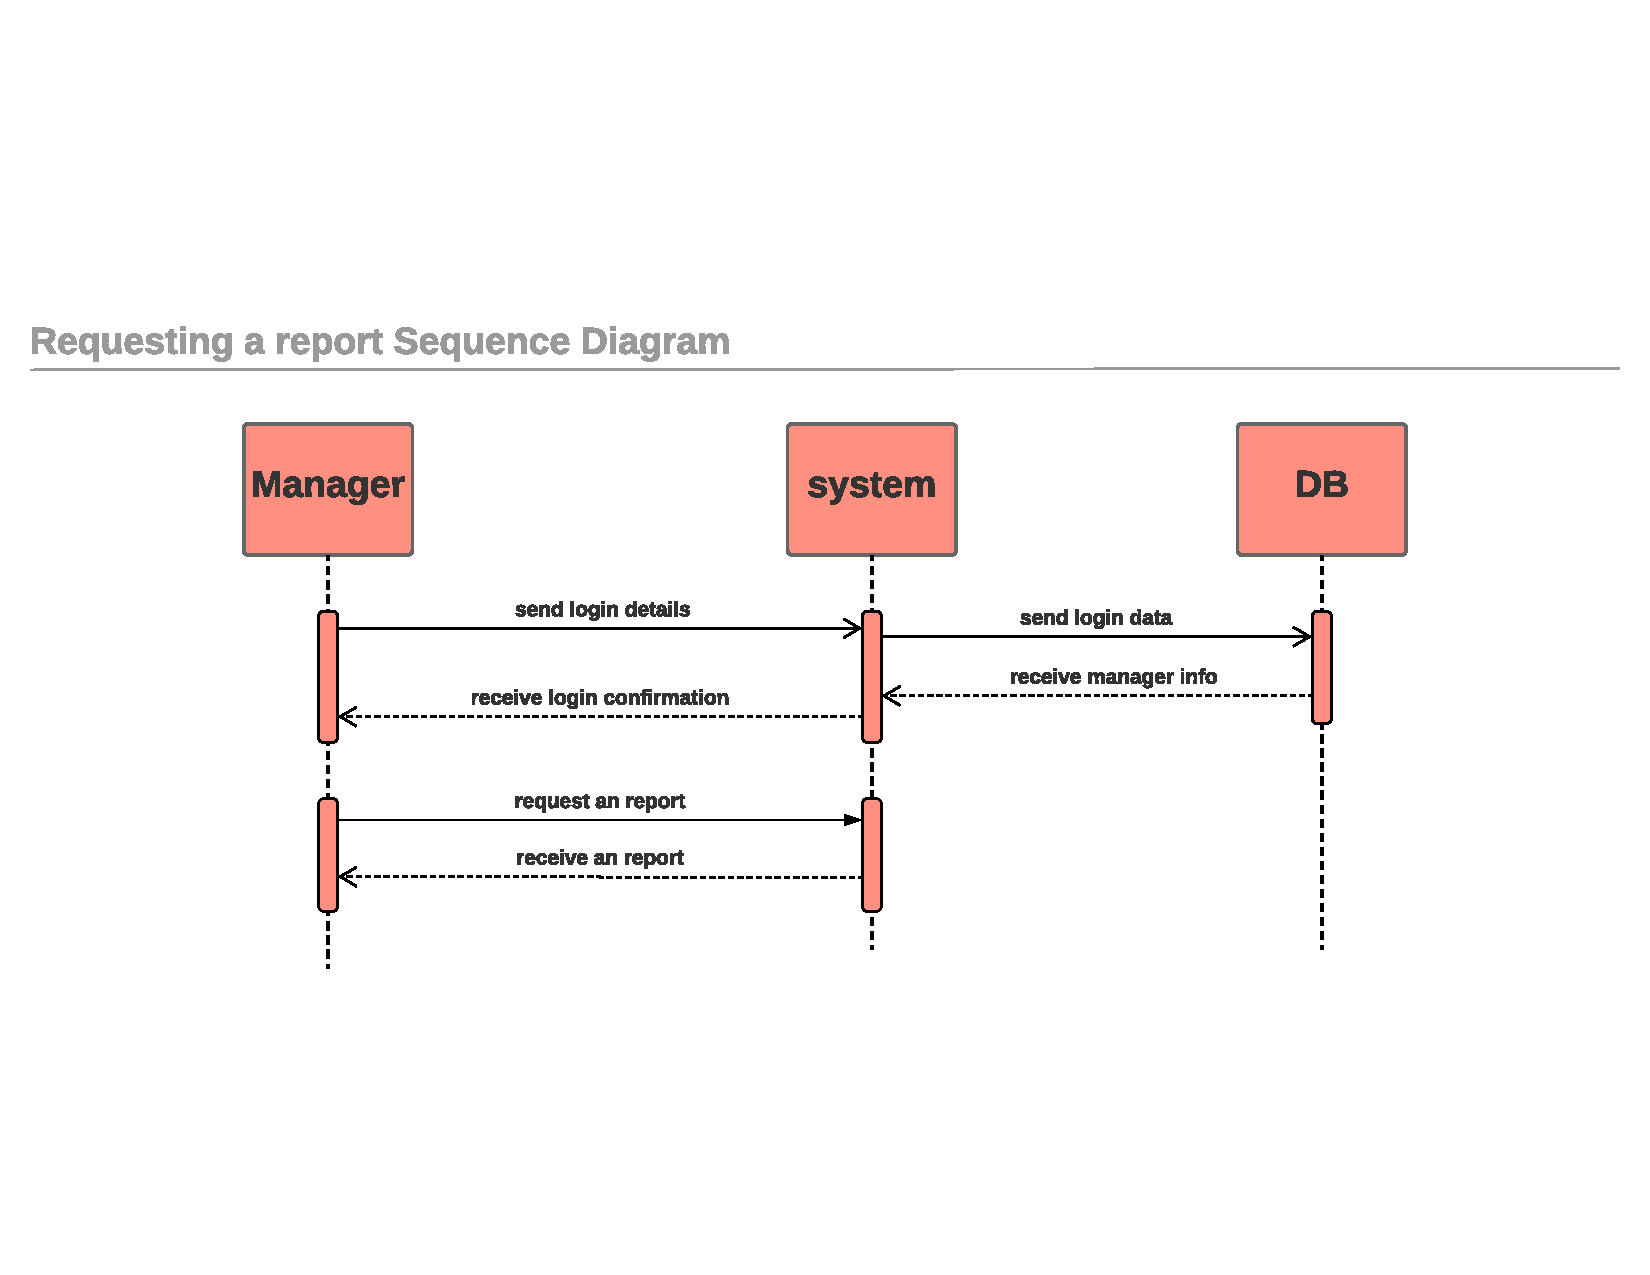
\includegraphics[width=\textwidth ,height=0.4\textheight ,scale=4]{Diagrams/sequence_diagram/manager_requesting_report.pdf}
								\label{FIG:2.13}
							
							
							
						\subsubsection{Revenue reports}
							
								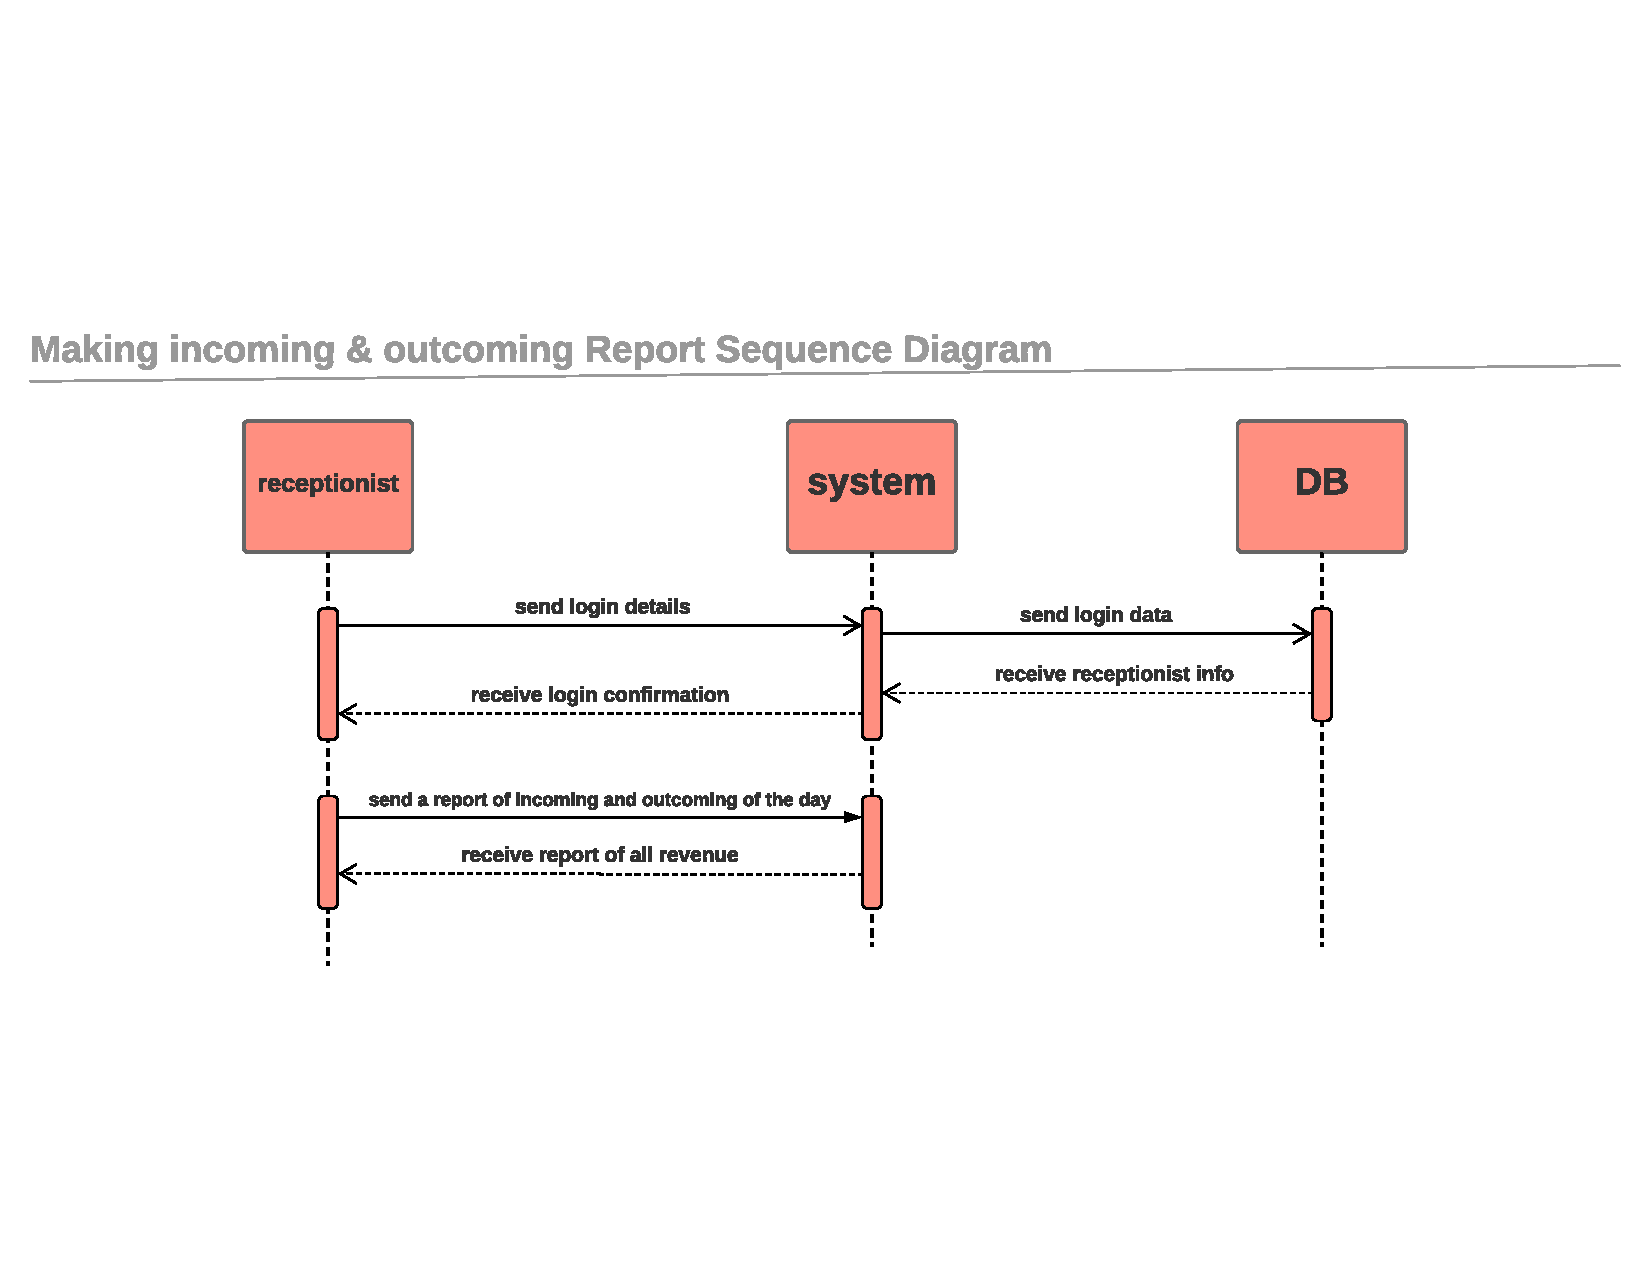
\includegraphics[width=\textwidth ,height=0.4\textheight ,scale=4]{Diagrams/sequence_diagram/report_of_revenue.pdf}
								\label{FIG:2.14}
							
							
							
						\subsubsection{Trainee unroll courses}
							
								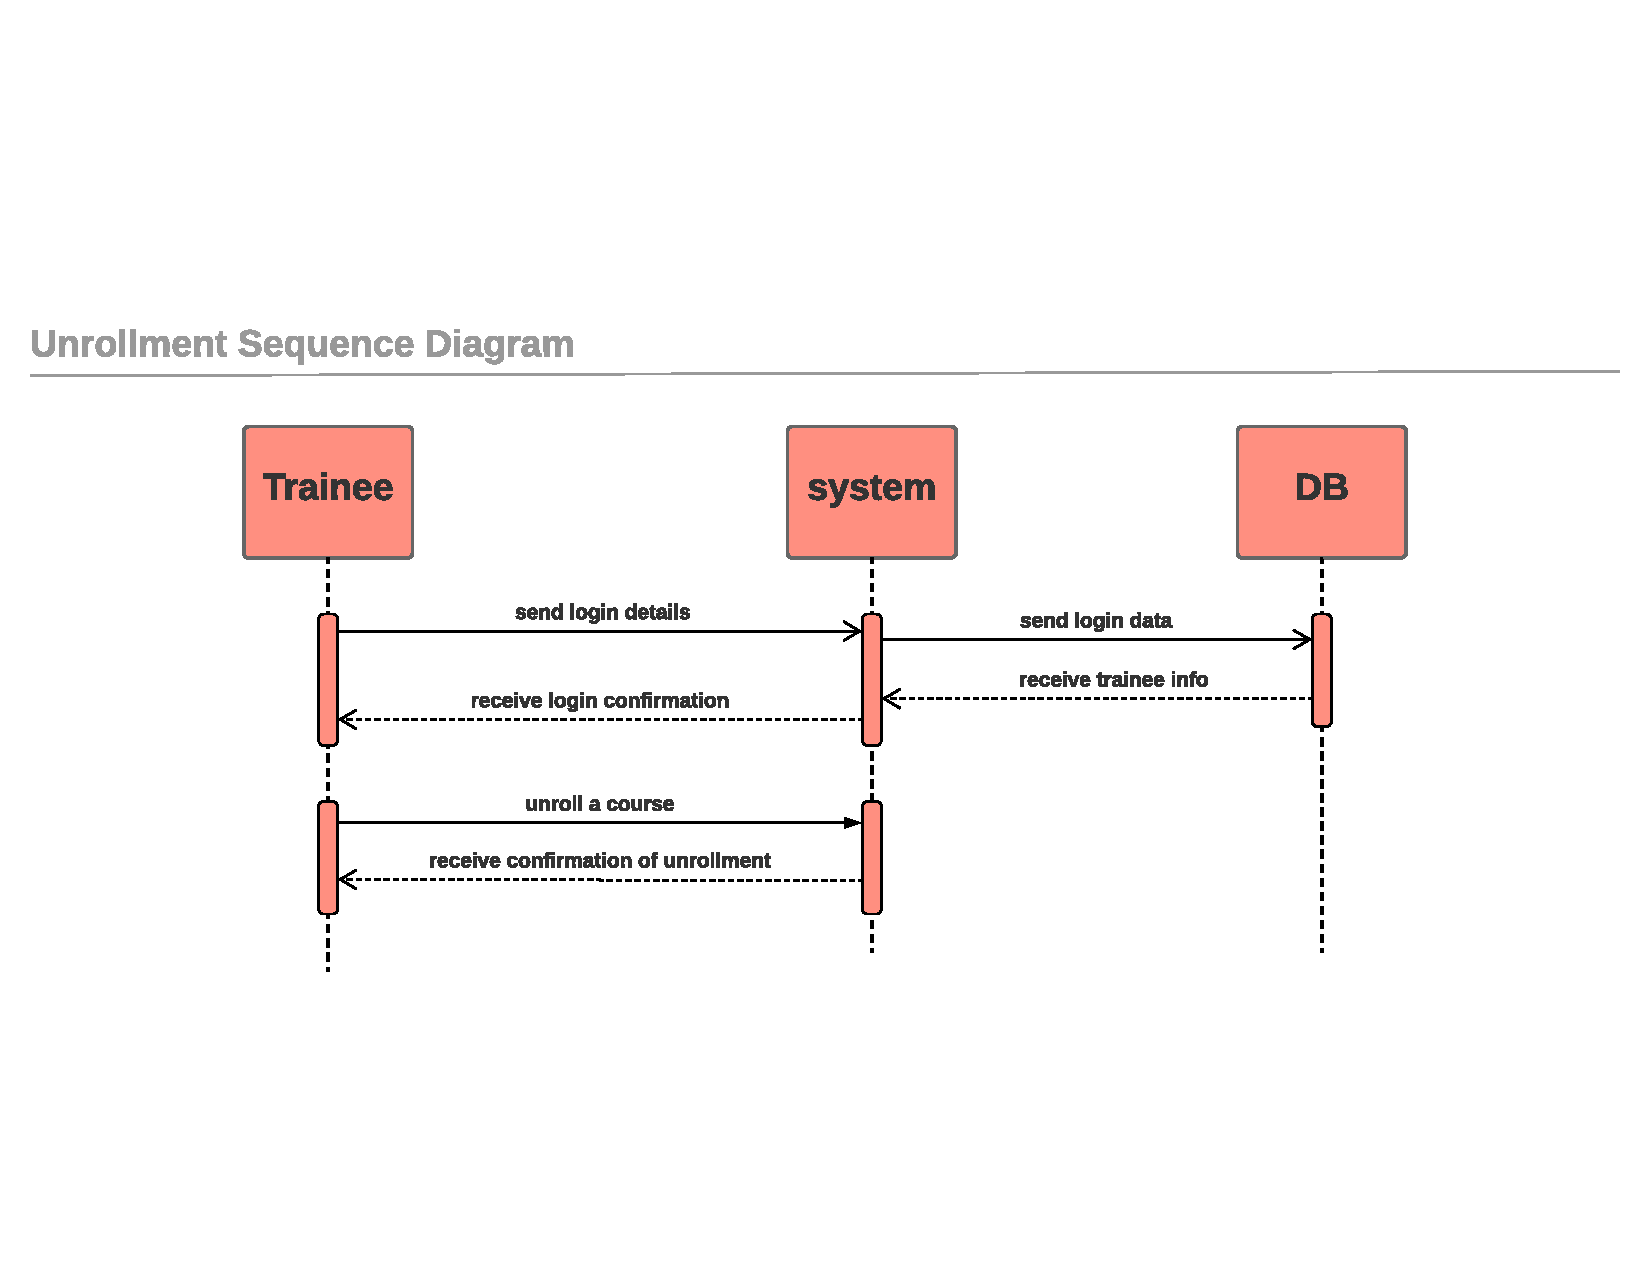
\includegraphics[width=\textwidth ,height=0.4\textheight ,scale=4]{Diagrams/sequence_diagram/unrollment.pdf}
								\label{FIG:2.15}
							
							
%%%%%%%%%%%%%%%%%%%%%%%%%%%%%%%%%%%%%%%%%%%%%%%%%%%%%%%%%%%%%%%%%%%%%%%%%%%%%%%%%%%%%%%%%%%%%%%%%%%%%%%%%%%%%%%%%%%%%%%%%%%%%%%%%%%%%%%%%%%%%%%%%%%%%%%%%%%%%%%%%%%%%%%%%%%%%%%%%%%%%%%%%%%%%%%%%%%%%%%%%%%%%%%%%%%%%%
		\section{ASSUMPTION DEPENDENCIES}
			\paragraph{Let us assume that this is an Inelegant psychological System and it is used in the following application:}
				\subsection{For Management system}
					\begin{itemize}
							\item
								\textbf{\textsc{\color{red}Manager}}
									\begin{itemize}
						\item
							\textbf{\textsc{\color{blue}connect with Employees and supervise them.}}
						\item
							\textbf{\textsc{\color{blue}connect with clients and monitoring motions of organization.}}
						\item
							\textbf{\textsc{\color{blue}veiw all reports that specified to Calculations and salaries of Employees and Exports resources ...etc.}}
						
					\end{itemize}
							\item
								\textbf{\textsc{\color{red}Receptionist stuff}}
									\begin{itemize}
										\item
											\textbf{\textsc{\color{blue}create an account for new user.}}
										\item
											\textbf{\textsc{\color{blue}make reservation of appointment or course to specific client.}}
										\item
											\textbf{\textsc{\color{blue}recourd sessions per day and help you in the calculations.}}
						
									\end{itemize}
					\end{itemize}
				
				\subsection{For clinic system}
				\begin{itemize}
					\item
							\textbf{\textsc{\color{red}client:}}
					\begin{itemize}
						\item
							\textbf{\textsc{\color{blue}A request for booking session with specific specialist.}}
						\item
							\textbf{\textsc{\color{blue}choosing from available appointments for his specialist.}}
						\item
							\textbf{\textsc{\color{blue}View his specific reports to his case and results, plans, and solving to issues that specified to his case.}}
						\item
							\textbf{\textsc{\color{blue}update or cancel his resrvation, and update his profile.}}
					\end{itemize}
					
					\item
							\textbf{\textsc{\color{red}Psychologist:}}
							\begin{itemize}
							\item
								\textbf{\textsc{\color{blue}Enter his appointments to the system.}}
							\item
								\textbf{\textsc{\color{blue}update and delete any appointment belongs to him, and update his profile.}}
							\item
								\textbf{\textsc{\color{blue}upload the reports that specified to his cases and upload his plan of treatment.}}
							\item
								\textbf{\textsc{\color{blue}connect with cases and receptionist.}}
					\end{itemize}
				\end{itemize}
				
				\subsection{For academic system}
				
					\begin{itemize}
					\item
							\textbf{\textsc{\color{red}Trainee:}}
					\begin{itemize}
						\item
							\textbf{\textsc{\color{blue}A request for booking course.}}
						\item
							\textbf{\textsc{\color{blue}choosing from available appointments for the course that he Enrolled it.}}
						\item
							\textbf{\textsc{\color{blue}system should rtrive to him his schedule.}}
						\item
							\textbf{\textsc{\color{blue}update or cancel his resrvation, and update his profile.}}
					\end{itemize}
					
					\item
							\textbf{\textsc{\color{red}Lecturer:}}
							\begin{itemize}
							\item
								\textbf{\textsc{\color{blue}Enter his appointments for the courses to the system.}}
							\item
								\textbf{\textsc{\color{blue}update and delete any appointment belongs to him, and update his profile.}}
							\item
								\textbf{\textsc{\color{blue}upload the reports of result that specified to his trianees and upload scoring to them.}}
							\item
								\textbf{\textsc{\color{blue}generate some tests and help trainer in correcting this tests.}}
					\end{itemize}
				\end{itemize}
		
%%%%%%%%%%%%%%%%%%%%%%%%%%%%%%%%%%%%%%%%%%%%%%%%%%%%%%%%%%%%%%%%%%%%%%%%%%%%%%%%%%%%%%%%%%%%%%%%%%%%%%%%%%%%%%%%%%%%%%%%%%%%%%%%%%%%%%%%%%%%%%%%%%%%%%%%%%%%%%%%%%%%%%%%%%%%%%%%%%%%%%%%%%%%%%%%%%%%%%%%%%%%%%%%%%%%%%
\end{document}